\documentclass[
	%fleqn,				% alinha todas as equações a esquerda
	12pt,				% tamanho da fonte
	openright,			% capítulos começam em pág ímpar (insere página vazia caso preciso)
	twoside,			% para impressão em verso e anverso. Oposto a oneside
	a4paper,			% tamanho do papel. 
	projeto,			% tipo do trabalho (opções: tcc, projeto)
]{cct-uenp}
% !TeX spellcheck = pt_BR
% ---
% PACOTES
% ---

% ---
% Pacotes fundamentais 
% ---
\usepackage[T1]{fontenc}		% Selecao de codigos de fonte.
\usepackage[utf8]{inputenc}		% Codificacao do documento (conversão automática dos acentos)
\usepackage{graphicx}			% Inclusão de gráficos
\usepackage{pdfpages}			% Inclusão de (páginas de) arquivos PDF no documento
\usepackage{amsmath}            % Pacote de elementos matemáticos da AMS
\usepackage{placeins}           % utilização do Floatbarrier para fixar imagem no local correto no documento
\usepackage{enumerate}
\usepackage{mathtools}
\usepackage{amssymb}
% ---
		
% ---
% Pacotes adicionais, usados apenas no âmbito do Modelo Canônico do abnteX2
% ---
\usepackage{lipsum}				% para geração de dummy text
% ---

\usepackage{multirow}
\usepackage{multicol}

\usepackage{tikz}
\usepackage{pgf}
\usetikzlibrary{automata,positioning,arrows.meta}
\usepackage[graphics,tightpage,active,pdftex]%{preview}
%\setlength{\PreviewBorder}{5pt}
%\PreviewEnvironment{tikzpicture}
% !TeX spellcheck = pt_BR

% ---
% Informações de dados para CAPA, FOLHA DE ROSTO e outros elementos
% ---
\titulo{Verificação formal aplicada a protocolos de rede}
\tituloingles{Formal verification applied on network protocols}
\palavraschave{Latex. Template ABNT. Editoração de texto.}
\palavraschaveingles{Latex. ABNT. Text editoration.}
\autor{Gustavo Oliveira Dias}
\citacaoautor{DIAS, G. O.}
\data{2017}

\diadefesa{24 de novembro}
\orientador{Prof. Me. Wellington A. Della Mura} % É membro nato e presidente da Banca Examinadora
% \coorientador{Prof(a). Dr(a). Nome do(a) Coorientador(a)} % Pode ou não ser membro da Banca; se for, deve ser incluído como membro a seguir
\membrobancadois{Prof. Dr. Segundo Membro da Banca}
\instmembrobancadois{Universidade/Instituição do Segundo Membro da Banca}
\membrobancatres{Prof. Dr. Terceiro Membro da Banca}
\instmembrobancatres{Universidade/Instituição do Terceiro Membro da Banca}
%\membrobancaquatro{Prof. Ms. Quarto Membro da Banca}
%\instmembrobancaquatro{Universidade/Instituição do Quarto Membro da Banca}

% ---
% Informações de dados para CAPA, FOLHA DE ROSTO e outros elementos
% ---
\titulo{Algoritmo para verificação formal do protocolo MQTT}
\tituloingles{Title of the Work}
\palavraschave{Latex. Template ABNT. Editoração de texto.}
\palavraschaveingles{Latex. ABNT. Text editoration.}
\autor{Gustavo Oliveira Dias}
\citacaoautor{DIAS, G. O.}
\data{2017}

\diadefesa{15 de Setembro}
\orientador{Prof. Me. Wellington Aparecido Della Mura} % É membro nato e presidente da Banca Examinadora
% \coorientador{Prof(a). Dr(a). Nome do(a) Coorientador(a)} % Pode ou não ser membro da Banca; se for, deve ser incluído como membro a seguir
\membrobancadois{Prof. Me. Carlos Eduardo Ribeiro}
\instmembrobancadois{Universidade Estadual do Norte do Paraná}
\membrobancatres{Prof. Dr. Bruno Squizato Faiçal}
\instmembrobancatres{Universidade Estadual do Norte do Paraná}


\makeindex % compila o indice

\begin{document}

% Retira espaço extra obsoleto entre as frases.
\frenchspacing 


%%%%%%%%%%%%%%%%%%%%%%%%%%%%%%%%%%%%%%%%%%%%%%%%%%%%%%%
\imprimircapa

\imprimirfolhaderosto*

\imprimirfolhadeaprovacao

%% !TeX spellcheck = pt_BR

% ----------------------------------------------------------
% ELEMENTOS PRÉ-TEXTUAIS
% ----------------------------------------------------------
% \pretextual

% ---
% Capa (elemento obrigatório)
% ---
\imprimircapa
% ---

% ---
% Folha de rosto (elemento obrigatório)
% (o * indica que haverá a ficha bibliográfica)
% ---
\imprimirfolhaderosto*
% ---

% ---
% Ficha bibliografica (elemento obrigatório para versões finais de TCC e dissertação)
% ---


% ---
% Folha de aprovação (elemento obrigatório) ==> deve ser omitida no caso de tccpreliminar
% ---

% Isto é um exemplo de Folha de aprovação, elemento obrigatório da NBR
% 14724/2011 (seção 4.2.1.3). Você pode utilizar este modelo até a aprovação
% do trabalho. Após isso, substitua todo o conteúdo deste arquivo por uma
% imagem da página assinada pela banca com o comando abaixo:
%
% \includepdf{folhadeaprovacao_final.pdf}
\imprimirfolhadeaprovacao
% ---

% ---
% Dedicatória (elemento opcional)
% ---
\begin{dedicatoria}
   \vspace*{\fill}
   \centering
   \noindent
   \textit{ Este trabalho é dedicado às crianças adultas que,\\
   quando pequenas, sonharam em se tornar cientistas.} \vspace*{\fill}
\end{dedicatoria}
% ---

% ---
% Agradecimentos (elemento opcional, mas fortemente recomendado)
% ---
\begin{agradecimentos}
Os agradecimentos principais são direcionados à Gerald Weber, Miguel Frasson,
Leslie H. Watter, Bruno Parente Lima, Flávio de Vasconcellos Corrêa, Otavio Real
Salvador, Renato Machnievscz\footnote{Os nomes dos integrantes do primeiro
projeto abn\TeX\ foram extraídos de
\url{http://codigolivre.org.br/projects/abntex/}} e todos aqueles que
contribuíram para que a produção de trabalhos acadêmicos conforme
as normas ABNT com \LaTeX\ fosse possível.

Agradecimentos especiais são direcionados ao Centro de Pesquisa em Arquitetura
da Informação\footnote{\url{http://www.cpai.unb.br/}} da Universidade de
Brasília (CPAI), ao grupo de usuários
\emph{latex-br}\footnote{\url{http://groups.google.com/group/latex-br}} e aos
novos voluntários do grupo
\emph{\abnTeX}\footnote{\url{http://groups.google.com/group/abntex2} e
\url{http://abntex2.googlecode.com/}}~que contribuíram e que ainda
contribuirão para a evolução do \abnTeX.

\end{agradecimentos}
% ---

% ---
% Epígrafe (elemento opcional)
% ---
\begin{epigrafe}
    \vspace*{\fill}
	\begin{flushright}
		\textit{``Não vos amoldeis às estruturas deste mundo, \\
		mas transformai-vos pela renovação da mente, \\
		a fim de distinguir qual é a vontade de Deus: \\
		o que é bom, o que Lhe é agradável, o que é perfeito.\\
		(Bíblia Sagrada, Romanos 12, 2)}
	\end{flushright}
\end{epigrafe}
% ---

% ---
% RESUMOS
% ---

% ---
% Resumo em Português (elemento obrigatório)
% ---
\begin{resumo}
 Segundo a \citeonline[3.1-3.2]{NBR6028:2003}, o resumo deve ressaltar o
 objetivo, o método, os resultados e as conclusões do documento. A ordem e a extensão
 destes itens dependem do tipo de resumo (informativo ou indicativo) e do
 tratamento que cada item recebe no documento original. O resumo deve ser
 precedido da referência do documento, com exceção do resumo inserido no
 próprio documento. (\ldots) As palavras-chave devem figurar logo abaixo do
 resumo, antecedidas da expressão Palavras-chave:, separadas entre si por
 ponto e finalizadas também por ponto.
\end{resumo}
% ---

% ---
% Resumo em Inglês (elemento obrigatório)
% ---
% O ambiente Abstract (com A maiúsculo) é definido no estilo dc-uel
\begin{Abstract}
 This is the english abstract. The Abstract in English should be faithful to the
 Resumo in Portuguese, but not a literal translation.
\end{Abstract}
% ---

% ---
% Lista de ilustrações (elemento opcional, mas fortemente recomendado)
% ---
\pdfbookmark[0]{\listfigurename}{lof}
\listoffigures*
\cleardoublepage
% ---

% ---
% Lista de tabelas (elemento opcional, mas fortemente recomendado)
% ---
\pdfbookmark[0]{\listtablename}{lot}
\listoftables*
\cleardoublepage
% ---

% ---
% Lista de abreviaturas e siglas (elemento opcional)
% ---
\begin{siglas}
  \item[ABNT] Associação Brasileira de Normas Técnicas
  \item[BNDES] Banco Nacional de Desenvolvimento Econômico e Social
  \item[IBGE] Instituto Nacional de Geografia e Estatística
  \item[IBICT] Instituto Brasileiro de Informação em Ciência e Tecnologia
  \item[NBR] Norma Brasileira
\end{siglas}
% ---

% ---
% Lista de símbolos (elemento opcional)
% ---
% \begin{simbolos}
%   \item[$ \Gamma $] Letra grega Gama
%   \item[$ \Lambda $] Lambda
%   \item[$ \zeta $] Letra grega minúscula zeta
%   \item[$ \in $] Pertence
% \end{simbolos}
% ---



% ---
% Sumario (elemento obrigatório)
% ---
\pdfbookmark[0]{\contentsname}{toc}
\tableofcontents*
\cleardoublepage
% ---
% ----------------------------------------------------------
% ELEMENTOS TEXTUAIS
% ----------------------------------------------------------
\textual
\pagestyle{uenp-header} % Configura cabeçalho para apresentar apenas números de página


% ----------------------------------------------------------
% Introdução
% ----------------------------------------------------------

\chapter{Introdução}

O termo Internet das Coisas, do inglês, \textit{Internet of Things} (IoT), foi usado pela primeira vez em 1998 para definir objetos do mundo físico representados virtualmente por meio de dispositivos interconectados~\cite{weber2010internet}. 

Advinda do avanço das áreas de sistemas embarcados, microeletrônica, comunicação e tecnologia de informações ~\cite{iot2016}, a IoT é considerada uma das mais promissoras tecnologias emergentes~\cite{gartner2015gartner}. Conforme o crescimento da quantidade de dispositivos e aplicativos conectados a \textit{Internet}, aumenta o interesse dos usuários em adquiri-los, tal como o de empresas em investir neste mercado~\cite{mukherjee2016ranking}.

Em estudo realizado pela \textit{Acquity Group}, mais de dois terços dos consumidores planejam comprar tecnologia conectada para suas casas até 2019~\cite{press2014internet}. Também, até 2017, 82\% das empresas implementarão a IoT de alguma forma, de acordo com relatório publicado pela \textit{Business Insider UK}~\cite{danova2014bi}.

Através da conexão e troca de mensagens entre os dispositivos, é possível realizar o monitoramento de ambientes controlados,  dispondo de uma vasta área de aplicações. Entre elas, pode-se destacar: carros, cidades e fazendas inteligentes; transporte e logística; cuidados médicos; interação pessoal e social; e processos industriais~\cite{sankarinternet, bandyopadhyay2011internet, atzori2010internet}.

Dentre os diversos fatores responsáveis pelo crescimento do interesse na área, ressalta-se a miniaturização do \textit{hardware}, além da criação do Protocolo de \textit{Internet} IPv6~\cite{press2014internet}. Capaz de alocar até $2^{128}$ endereços IP, o IPv6 possibilita a conexão de uma imensa quantidade de dispositivos~\cite{mukherjee2016ranking}.

Segundo a Cisco, até 2020 haverá cerca de 50 bilhões de dispositivos conectados, e até 2022, o mercado de soluções para IoT acrescentará em torno de 14,4 trilhões de dólares ao PIB global~\cite{morgan2014forbes}.

De forma geral, dispositivos utilizados em IoT possuem recursos limitados de memória e processamento, além de operarem em ambientes com baixa largura de banda ou redes instáveis ~\cite{weber2010internet, iot2016, suo2012security}. Portanto, é essencial que a comunicação e a troca de dados entre eles seja executada da forma eficiente, sendo este, um dos principais desafios enfrentados em IoT~\cite{bandyopadhyay2011internet, suo2012security}.

Devido as suas características, as aplicações de IoT necessitam de padronizações específicas. Logo, tratando-se estritamente da comunicação entre os dispositivos, foi desenvolvido em 1999 pela IBM e Eurotech o protocolo MQTT (\textit{Message Queue Telemetry Transport protocol})~\cite{mqttv3.1}. 

Padronizado em 2014 pela OASIS~\cite{mqttv3.1.1}, o MQTT tem como principal objetivo minimizar o uso de largura de banda da rede e recursos dos dispositivos. Para isso, o protocolo foi desenvolvido com base em diversos conceitos que asseguram uma alta taxa de entrega das mensagens~\cite{chen2014responsive}.

Com o advento do MQTT, suas propriedades e aplicações tornaram-se alvo de pesquisas, a fim de encontrar vulnerabilidades, ambiguidades e inconsistências, contribuindo com o aprimoramento da tecnologia~\cite{aziz2016formal, mladenov2017formal}.

Diversos métodos são utilizados por especialistas para verificação e validação de propriedades de protocolos e sistemas complexos, entre eles, destaca-se: simulação, teste de protótipo, verificação dedutiva e verificação formal~\cite{clarke1999model}. 

Com exceção da verificação formal, os demais métodos, embora sejam amplamente usados, não garantem total ausência de erros no funcionamento do sistema, uma vez que são incapazes de checar de forma automática todos os caminhos possíveis, visto que dependem de decisões humanas acerca de quais pontos devem ser analisados, tornando-os suscetíveis a falhas~\cite{clarke1999model}. 

Ademais, tais métodos apresentam deficiências que podem envolver tempo excessivo para análise e observação, além de gastos elevados com especialistas encarregados de aplicá-los~\cite{clarke1999model}.

A verificação formal engloba a técnica de teste baseado em modelo, também conhecida como \textit{Model Checking}, a qual proporciona uma série de vantagens em comparação com os outros métodos, tais como aplicação automática, verificação completa de todos os caminhos possíveis e produção de contraexemplos que demonstram quando uma dada propriedade não é satisfeita. Além disso, não é necessário a especificação completa do sistema, uma vez que seus módulos podem ser representados separadamente. Assim, pode-se verificar apenas os pontos críticos, poupando tempo e provendo maior segurança e confiabilidade~\cite{clarke1999model}.

Portanto, este trabalho tem como objetivo desenvolver um algoritmo para verificação formal da versão 3.1.1 do protoclo MQTT e suas propriedades por meio de \textit{Model Checking}.

O algoritmo será implementado e testado por meio de um estudo de caso. Com isso, espera-se que a comunicação entre dispositivos nos projetos de IoT que utilizam o protocolo MQTT possa ser verificada antes de sua implantação.

\section{Motivação}

Como dito anteriormente, a Internet das Coisas é uma das mais poderosas tecnologias emergentes, estima-se que até 2022 ela irá adicionar de 14,4 trilhões de dólares ao PIB global, e que em 2020 haverá em torno de 50 bilhões de dispositivos interconectados~\cite{morgan2014forbes}, aumentando a demanda por sensores, dispositivos de rede sem fio, serviços de armazenamento em nuvem, entre outros serviços e dispositivos que compõem este ambiente tecnológico, despertando assim, o interesse dos setores industriais e acadêmicos.

A comunicação é um fator crítico num projeto em IoT, pois a troca de dados e informações entre os dispositivos é essencial para seu sucesso. Com a heterogeneidade de dispositivos que compõem o ambiente, padronizações são necessárias para manter a interoperabilidade entre os mesmos, sendo essa uma das funções que os protocolos pretender cumprir.

O protocolo MQTT foi desenvolvido especialmente para aplicações em IoT e M2M (\textit{Machine-to-Machine}). Com um cabeçalho de apenas 2 \textit{bytes}, e implementando um servidor próprio, chamado de \textit{broker}, é capaz de prover a troca de mensagens entre dispositivo por meio da estratégia \textit{publish/subscribe}, minimizando o uso de banda de rede e recursos do dispositivo~\cite{mqttv3.1.1}. 

\begin{figure}[ht]
	\centering
	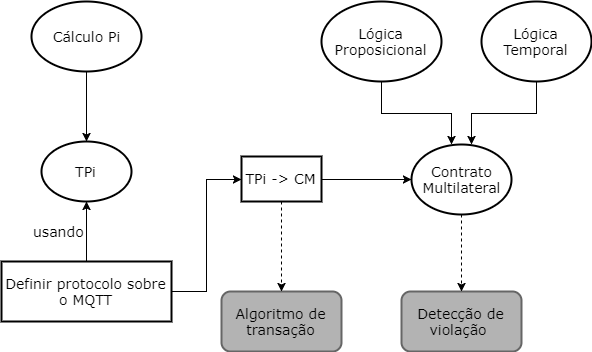
\includegraphics[width=1\textwidth]{imagens/tcc_estrutura.png}
	\caption{Escopo do método proposto.
		\label{fig:tcc_escopo}}
\end{figure}
\FloatBarrier

\section{Formulação e Escopo do Problema}

Como relatado acima, não se tem conhecimento de alguma ferramenta baseada em verificação formal que permita modelar a comunicação entre os dispositivos de projetos em IoT, assim como realizar a checagem automática de suas propriedades. Em vista disso, a principal questão a ser respondida é:

\textbf{É possível modelar e verificar a comunicação entre dispositivos que utilizam o protocolo MQTT?}

No intuito de responder essa questão, a resolução das seguintes subquestões devem ser fornecidas:

\textbf{\textit{(1) É possível modelar o MQTT?}}


No estudo desenvolvido por~\citeauthor{aziz2016formal}, e que serve de base para este trabalho, o protocolo é modelado através de uma álgebra temporal de processos, chamada \textit{TPi}.

\textbf{\textit{(2) É possível realizar a verificação formal do MQTT?}}

A partir do elaborado por~\citeauthor{aziz2016formal}, pode-se criar um algoritmo baseado em \textit{Model Checking} que faça a verificação de suas propriedades, o que leva ao objetivo do trabalho.

\section{Objetivos gerais e específicos}


\chapter{Fundamentação Teórica}\label{capitulo:fundamentacao}

Este capítulo apresenta alguns conceitos envolvendo IoT, como suas características, tecnologias envolvidas, poder de mercado e aplicações. A comunicação em IoT é discutida mais profundamente e os principais protocolos de comunicação são descritos e discutidos, em especial o MQTT, foco de pesquisa deste trabalho. Algumas representações para contratos eletrônicos, sistemas e processos concorrentes também são descritas, fornecendo um conjunto de conceitos necessários para a solução dos problemas propostos neste trabalho.

\section{Internet das Coisas}

Com o popularização das tecnologias de comunicação (\textit{Wi-Fi, \textit{Bluetooth}, 3G/4G, etc}), dos dispositivos conectados a \textit{internet}, juntamente com a difusão do IPv6, uma série de aplicações e tecnologias passam a ser exploradas.

Neste contexto, surge o conceito de Internet das Coisas, caracterizado por dispositivos inseridos na rede mundial de computadores para adquirir e trocar dados que devem ser processados, gerando informação e conhecimento que auxilia na tomada de decisões. 

Pode-se destacar a heterogeneidade como uma das principais características da IoT, pois promove a integração de diversos tipos de dispositivos e tecnologias, como sensores, dispositivos de rede, \textit{smartphones}, bancos de dados, protocolos, entre outros.

Em seu trabalho,~\citeauthor{mayer2009security} classifica a IoT em 8 tópicos:

\begin{itemize}
    \item \textbf{Comunicação:} permiti a troca de informações entre dispositivos;
    \item \textbf{Sensores:} captura e representa o mundo físico no mundo digital;
    \item \textbf{Atuadores:} realiza ações no mundo físico desencadeadas no mundo digital;
    \item \textbf{Armazenamento:} coleta de dados a partir de sensores, sistemas de identificação e rastreamento;
    \item \textbf{Dispositivos:} provê interação com humanos no mundo físico;
    \item \textbf{Processamento:} fornece mineração de dados e serviços;
    \item \textbf{Localização e rastreamento:} determinação e rastreamento de localização do mundo físico;
    \item \textbf{Identificação:} concede uma única identificação física de um objeto no mundo digital.
\end{itemize}

\begin{figure}[ht]
\centering
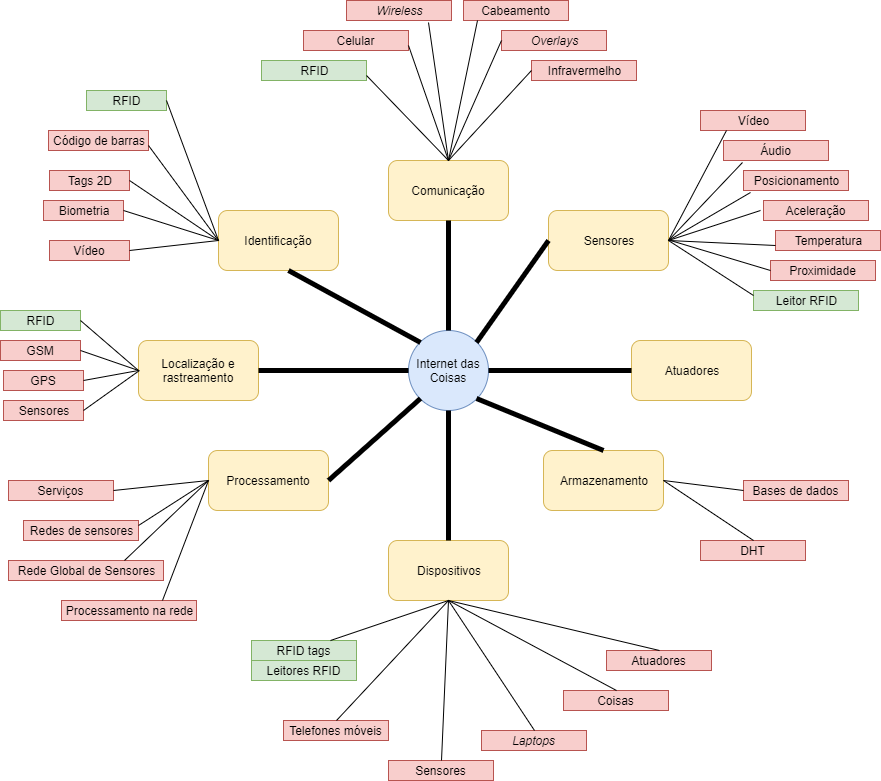
\includegraphics[width=1\textwidth]{imagens/iot_diagram.png}
\caption{Categorização dos tópicos e tecnologias em IoT~\cite{mayer2009security}, adaptado pelo autor.
\label{fig:iot_diag}}
\end{figure}
\FloatBarrier

A Internet das Coisas é um paradigma que desempenha e continuará desempenhando um papel vital num futuro próximo~\cite{sankarinternet}. \citeauthor{sankarinternet} classificam a IoT sob a perspectiva de visão, destacando três categorias: visão orientada a coisas; visão orientada a \textit{internet}; e visão orientada a semântica. Os paradigmas de visão são expostos na Figura~\ref{fig:iot_vision}.

\textbf{Visão Orientada a Coisas:} realiza o rastreamento ou monitoramento de objetos usando sensores e tecnologias ubíquas. O Código de Produto Eletrônico, do inglês \textit{Electronic Product Code} (EPC), costumava se usado para identificar objetos, e tal técnicas foi estendidas para os sensores.

\textbf{Visão Orientada a Internet:} objetos físicos são convertidos em objetos inteligentes. Um protocolo de \textit{internet} é atribuído a um objeto, que é acessado de forma exclusiva. O objeto habilitado pelo sensor torna-se inteligente, o qual é identificado exclusivamente e monitorado de forma contínua.

\begin{figure}[ht]
\centering
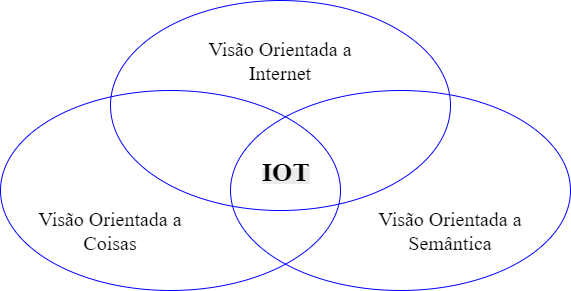
\includegraphics[width=0.7\textwidth]{imagens/iot_vision.png}
\caption{Três paradigmas de visão para IoT~\cite{sankarinternet}, adaptado pelo autor.
\label{fig:iot_vision}}
\end{figure}
\FloatBarrier

\textbf{Visão Orientada a Semântica:} tem-se uma grande quantidade de objetos habilitados por sensores conectados a \textit{internet}. Os sensores monitoram e geram continuamente os dados, que podem ser redundantes, além de serem heterogêneos ou homogêneos. A visão semântica ajuda a processar os dados de forma significativa e tomar as decisões necessárias adequadamente.

\subsection{Aplicações}

As potencialidades oferecidas pela IoT possibilitam uma vasta área de aplicações, das quais poucas são realmente aplicadas e comercializadas. Tais aplicações proverão maior eficiência e conforto em atividades como: fazer uma viagem de carro, cuidar da saúde, cultivar vegetais, trabalhar, malhar, entre muitas outras~\cite{bandyopadhyay2011internet, atzori2010internet}.

Estes ambientes podem ser equipados com objetos que comunicam-se para produzir informações de acordo com a percepção do ambiente ao redor. Isso implica numa gama de aplicações que podem ser desenvolvidas. Algumas destas são agrupadas nos seguintes tópicos:

\begin{itemize}
    \item \textbf{Transporte e logística:} Carros, aviões, ônibus, navios, bicicletas, estradas, portos e trilhos tornam-se mais monitoráveis com o uso de sensores, atuadores e processamento de dados. Assim, os meios para transporte e os bens transportados enviam informações para sistemas de controle de tráfego e de veículos para melhor direcionamento do trânsito, ajudando no controle e status das entregas e na exibição de informações aos motoristas acerca do tráfego~\cite{atzori2010internet}.
    \item \textbf{Saúde conectada:} Considerada uma revolução na área da medicina, envolve a coleta de dados por meio de sensores fixados ao corpo dos pacientes. Os dados são enviados para sistemas que realizam o monitoramento remoto da saúde. Deste modo, informações sobre a saúde dos pacientes podem ser vistas remotamente pelos seus familiares, pelos médicos e pelo próprio paciente~\cite{sankarinternet}.
    \item \textbf{Domínio pessoal e social:} Aplicações com objetivo de motivar o usuário a manter e construir novas relações pessoais. Mensagens podem ser enviadas para que as pessoas saibam o que os amigos estão fazendo, quais seus gostos em comum e demais informações. O domínio pessoal pode envolver, por exemplo, o rastreamento de objetos pessoais em caso de perda ou roubo~\cite{atzori2010internet}.
    \item \textbf{Ambientes inteligentes:} Carros conectados que emitem alertas de segurança ao motorista. Fazendas com sistemas de agropecuária e agricultura de precisão, visando aumentar a produção utilizando menos tempo e recursos. Processos industriais monitorados para maior eficácia na realização dos procedimentos. Casas conectadas, onde o morador pode controlar o funcionamento de eletrodomésticos, luzes, eletroeletrônicos e demais aparelhos, provendo conforto e qualidade de vida~\cite{sankarinternet, bandyopadhyay2011internet, atzori2010internet}. Todos os casos acima são exemplos de como a IoT pode auxiliar no aperfeiçoamento de processos envolvendo diversos ambientes. 
\end{itemize}

\begin{figure}[ht]
\centering
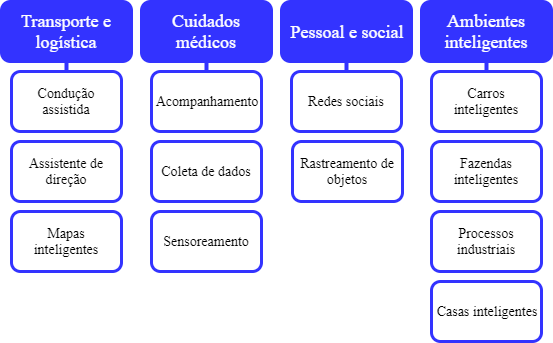
\includegraphics[width=0.9\textwidth]{imagens/iot_fields.png}
\caption{Áreas de aplicação e principais contextos~\cite{atzori2010internet}, adaptado pelo autor.
\label{fig:iot_fields}}
\end{figure}
\FloatBarrier

\section{Protocolos de comunicação}

Perante a perspectiva da comunicação, a Internet das Coisas pode ser vista como um conjunto de diferentes redes, incluindo redes móveis (3G, 4G, etc.), \textit{WLANs}, redes de sensores e redes \textit{Adhoc} móveis~\cite{buyya2016internet}.

Sendo assim, nota-se a existência de uma série de protocolos de comunicação disponíveis, considerando as diferentes tipos de redes que podem ser usadas. Logo, a escolha de um protocolo pode afetar diretamente fatores como a velocidade, confiabilidade e durabilidade de uma conexão.

Na Figura~\ref{fig:iot_protocols}, alguns protocolos são exibidos de acordo com a camada no qual é aplicado de acordo com o modelo \textit{TCP/IP}.

\begin{figure}[ht]
\centering
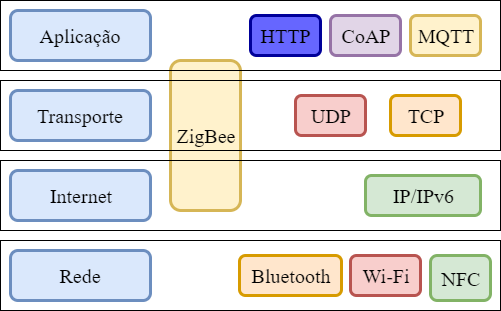
\includegraphics[width=0.7\textwidth]{imagens/iot_protocols.png}
\caption{Uso dos protocolos de acordo com a camada \textit{TCP/IP}~\cite{buyya2016internet}, adaptado pelo autor.
\label{fig:iot_protocols}}
\end{figure}
\FloatBarrier

No entanto, alguns protocolos que são amplamente usados em redes predominantemente formada por Computadores Pessoais, como o \textit{Internet Protocol version 6 (IPv6)} e o \textit{Hypertext Transfer Protocol (HTTP)}, não possuem a mesma usabilidade para a IoT, devido ao poder computacional restrito dos dispositivos~\cite{iot2016}.

O protocolo \textit{IPv6} representa um passo importante na evolução da IoT, visto que utiliza 128 bits para endereçamento de uma imensa quantidade de objetos, ante aos 32 bits utilizados pelo \textit{IPv4}. Entretanto, o \textit{IPv6} não se adequa as limitações de grande parte dos dispositivos aplicados na IoT. Por exemplo, enquanto que o \textit{IPv6} necessita de 1280 bytes de \textit{MTU}, dispositivos que seguem o padrão IEEE 802.15.4 (\textit{LR-WPANs}) limitam-se a pacotes de 128 bytes~\cite{iot2016}.

Objetivando resolver esses problemas, o \textit{IETF} desenvolveu o \textit{6LoWPAN}, uma camada de adaptação desenvolvida primordialmente para o padrão IEEE 802.15.4. Sua principal finalidade consiste na compressão de pacotes \textit{IPv6} utilizando informações de protocolos presentes em outras camadas, como o endereço MAC, por exemplo. Desta forma, permite o uso do \textit{IPv6} por dispositivos com baixo poder computacional~\cite{kushalnagar2007ipv6}.

Outro protocolo extensamente utilizado, mas que mostra-se inadequado para aplicações em IoT é o HTTP~\cite{iot2016}. Porém, os protocolos CoAP (\textit{Constrained Application Protocol}) e MQTT (\textit{Message Queue Telemetry Transport}), ideais para aplicações em IoT, foram desenvolvidos para lidar com a comunicação entre dispositivos com limitações de processamento inseridos em ambientes com redes instáveis e baixa largura de banda. 

As características gerais do HTTP serão discutidas na Seção~\ref{sec:http} a seguir. Adiante, nas Subseções~\ref{sec:coap} e~\ref{sec:mqtt}, serão abordadas características gerais do protocolo CoAP (\textit{Constrained Application Protocol}) e propriedades gerais e específicas do MQTT (\textit{Message Queue Telemetry Transport}), respectivamente. Por ser um dos principais focos de estudo deste trabalho, o MQTT será discutido com maior profundidade em relação ao HTTP e ao CoAP.

Por fim, a Seção~\ref{sec:protocols} exibe um breve comparativo entre as características gerais dos três protocolos em relação a usabilidade para IoT. 

\subsection{HTTP}\label{sec:http}

O protocolo HTTP é utilizado na camada de aplicação para receber e enviar informações na rede mundial de computadores usando a estratégia requisição/resposta sobre o paradigma cliente/servidor~\cite{fielding2014hypertext}, como pode ser observado na figura~\ref{fig:req/res}.

Utilizado em sistemas de informação de hipermídia, distribuídos e colaborativos, o HTTP prove comunicação por meio da troca ou transferência de hipertexto, que é um texto estruturado que utiliza ligações lógicas (\textit{hiperlinks}) entre nós contendo texto~\cite{fielding2014hypertext}.

A comunicação entre o cliente e o servidor é feita mediante a  mensagens, que são codificadas por meio da linguagem de marcação HTML~\cite{raggett1999html}. O cliente envia uma mensagem de requisição de um determinado recurso ao servidor, que recebe e requisição e enviar uma resposta, como ilustrado na Figura~\ref{fig:req/res}. As mensagens possuem cabeçalho e corpo, além de um método, no caso das mensagens de requisição~\cite{fielding2014hypertext}. Os principais métodos são listados abaixo:
\begin{itemize}
    \item \textbf{GET:} Solicita a exibição de um recurso;
    \item \textbf{POST:} Envia informações do corpo da requisição que serão utilizadas para criar um novo recurso;
    \item \textbf{DELETE:} Remove um recurso;
    \item \textbf{PUT:} Atualiza um recurso na URI (\textit{Uniform Resource Identifier}) especificada. Se o recurso não existir, o mesmo pode ser criado;
    \item \textbf{HEAD:} Retorna informações sobre um recurso.
\end{itemize}

\begin{figure}[ht]
\centering
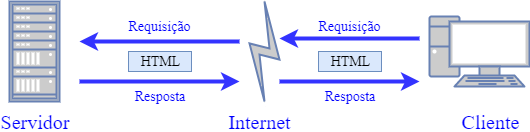
\includegraphics[width=0.8\textwidth]{imagens/cliente_servidor.png}
\caption{Estratégia requisição/resposta sobre o paradigma cliente/servidor.
\label{fig:req/res}}
\end{figure}
\FloatBarrier

O cabeçalho da mensagem HTTP é usado para transmitir mensagens adicionais entre o cliente e o servidor. Ele é especificado imediatamente após a linha inicial da transação que contêm o método, tanto para a requisição do cliente quanto para a resposta do servidor. Existem quatro tipos de cabeçalhos que podem ser incluídos nas mensagens~\cite{fielding2014hypertext}, os quais são:
\begin{itemize}
	\item \textbf{\textit{General-header}}: Utilizado para enviar informações adicionais sobre a mensagem transmitida;
	\item \textbf{\textit{Request-header}}: Presente em mensagens de requisição, permite ao cliente transmitir informações adicionais relacionadas à requisição, ao próprio cliente ou ao servidor;
	\item \textbf{\textit{Entity-header}}: Pode estar presente tanto em uma requisição quanto numa resposta. Usado para definir meta-dados sobre o corpo da mensagem, como tamanho, tipo e linguagem. Quando não há corpo na mensagem, os meta-dados referem-se aos recursos identificados pela requisição.
	\item \textbf{\textit{Response-header}}: Utilizado para transmitir informações adicionais da resposta. As informações podem estar relacionadas com o servidor ou sobre acesso adicional ao recurso identificado pelo \textit{Request}-URI.  
\end{itemize}

Uma mensagem mensagem HTTP pode conter um corpo de dados que são inseridos abaixo das linhas de cabeçalho.Em uma mensagem de resposta, o corpo da mensagem é o recurso que foi requisitado pelo cliente, ou ainda uma mensagem de erro, caso este recurso não seja possível. Já em uma mensagem de requisição, o corpo pode conter dados que serão enviados diretamente pelo usuário ou um arquivo que será enviado para o servidor~\cite{fielding2014hypertext}.

A Figura~\ref{fig:http_ex} apresenta um exemplo de requisição e resposta HTTP. À esquerda, é apresentado uma requisição, em que a primeira linha contêm o método da requisição (POST), a URI ("\textit{/servlet/default.jsp}") e a versão do protocolo ("\textit{HTTP/1.1}"). A linha de requisição é seguida por uma série de informações adicionais do cabeçalho, e por fim, na última linha, a informação "\textit{LastName=Magalhaes\&FirstName=Guilherme}" pertence ao corpo da mensagem. No exemplo de resposta HTTP, localizado à direita, a primeira linha armazena o status do protocolo~\cite{fielding2014hypertext}, com informações acerca da versão do protocolo ("HTTP/1.1"), o status do código ("\textit{200}" = bem sucedido) e uma \textit{Reason-Phrase}~\cite{fielding2014hypertext} ("\textit{OK}") que indica uma breve descrição textual sobre o status do código. Posterior a linha de status tem-se as informações do cabeçalho, que é semelhante as da requisição. Afinal, o corpo da resposta é o conteúdo HTML da própria resposta. 

\begin{figure}[ht]
	\centering
	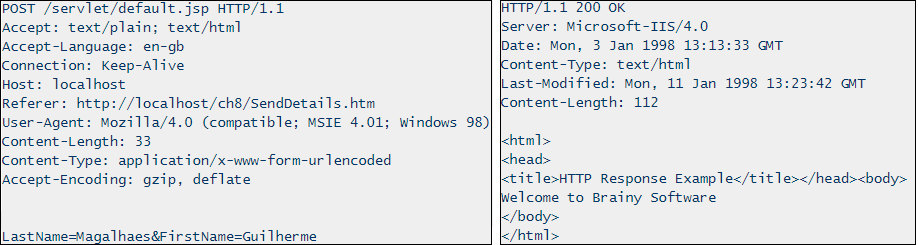
\includegraphics[width=0.8\textwidth]{imagens/ex_http.png}
	\caption{Exemplo de requisição e resposta HTTP.
		\label{fig:http_ex}}
\end{figure}
\FloatBarrier 

\subsection{CoAP}\label{sec:coap}

Definido em 2010 pela IETF, o CoAP tounou-se um \textit{Request for Comments} (\textit{RFC}) em 2014~\cite{shelby2014constrained}. Inicialmente, um grupo de trabalho criado pela IETF chamado \textit{Constrained RESTful Environments} (\textit{CoRE}) iniciou suas atividades em 2010 com o objetivo de desenvolver um \textit{framework} para aplicações que manipulam recursos simples localizados em dispositivos interconectados por meio de redes limitadas~\cite{shelby2014constrained}. 

Tais aplicações vão desde monitoramento de temperatura e medidores de energia por meio sensores, até o controle de atuadores como interruptores ou trancas eletrônicas, além do gerenciamento de dispositivos que compõem a rede. Assim sendo, o CoAP trata de uma parte deste \textit{framework}~\cite{shelby2014constrained}.

Segundo o RFC 7252~\cite{shelby2014constrained}, o CoAP é um protocolo de comunicação voltado para objetos limitados (com pouca memória \texttt{RAM}, por exemplo) e redes restritas onde há frequente perda de pacotes. Projetado para aplicações \textit{Machine-to-Machine} (\texttt{M2M}), o CoAP define quatro tipos de mensagens:
\begin{itemize}
    \item \textbf{\textit{Confirmable (CON)}:} Mensagens que precisam ser confirmadas no destino. Se não houver perda de pacotes, cada mensagem deste tipo resulta em uma mensagem do tipo \textit{Acknowledgment} ou \textit{Reset};
    \item \textbf{\textit{Non-confirmable (NON)}:} Mensagem que não necessita de confirmação de recebimento.
    \item \textbf{\textit{Acknowledgment (ACK)}:} Confirmação de uma mensagem \textit{Confirmable}.
    \item \textbf{\textit{Reset (RST)}:} Indica que outra mensagem CON ou NON foi recebida, mas não pôde ser processada devido a falta de algum contexto.
\end{itemize}

O CoAP oferece uma estratégia de interação requisição/resposta entre os dispositivos das aplicações e inclui recursos \textit{Web} como URIs e tipos de mídias usadas na \textit{Internet}, além de interagir com o HTTP para integração com a \textit{Web}. Outras características descritas no RFC 7252~\cite{shelby2014constrained} são citadas abaixo:
\begin{itemize}
    \item Troca de mensagens assíncrona;
    \item Capacidades simples de \textit{proxy} e \textit{caching};
    \item Mapeamento HTTP que permite que \textit{proxies} possam prover acesso aos recursos do CoAP via HTTP;
    \item Interligação segura para \textit{Datagram Transport Layer Security} (DTLS);
    \item \textit{Binding} em \textit{Datagram Transport Layer Security} (UDP) com confiabilidade opcional suportando requisições tanto \textit{unicast} quanto \textit{multicast};
    \item Suporte aos métodos GET, POST, PUT e DELETE.
de maneira uniforme
\end{itemize}

\begin{figure}[ht]
\centering
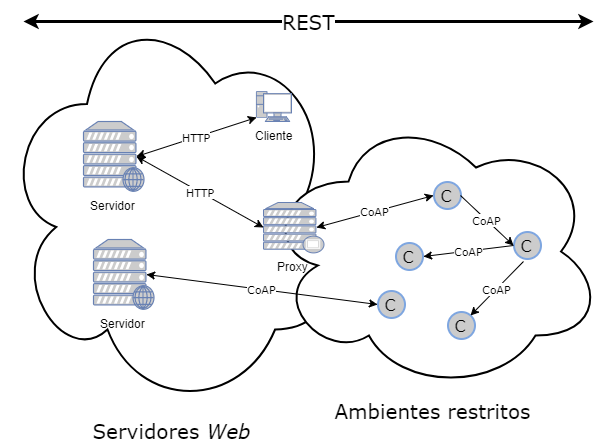
\includegraphics[width=0.8\textwidth]{imagens/coap_arq.png}
\caption{Arquitetura CoAP~\cite{shelby2014constrained}.
\label{fig:coap_arq}}
\end{figure}
\FloatBarrier
 
 A Figura~\ref{fig:coap_arq} apresenta uma abstração da arquitetura CoAP. Um dos objetivos do CoRE embasa-se em adequar a arquitetura \textit{Representational State Transfer} (REST) para ambientes restritos aos nós e rede, e, baseado nisso, foi desenvolvido o CoAP. Sendo assim, o CoAP pode ser considerado um protocolo \textit{RESTfull}~\cite{shelby2014constrained}.
 
 A comunicação com o CoAP consiste na troca de mensagens compactas transportadas sobre o UDP, sendo que, há uma camada DTLS entre as mensagens e o UDP, usada para prover segurança aos dados~\cite{shelby2014constrained}. 
 
 As mensagens são codificadas em formato binário com um cabeçalho fixo de 4 \textit{bytes}, seguido de um \textit{token} com largura variável (de 0 a 8 \textit{bytes}). Após o \textit{token} pode haver ou não uma série de opções do CoAP no formato \textit{Type-Length-Value} (TLV). As opções TLV podem ser seguidas por um \textit{payload}, preenchendo o resto o do datagrama~\cite{shelby2014constrained}. O formato da mensagem é ilustrado na Figura~\ref{fig:coap_header}.
 
 \begin{figure}[ht]
\centering
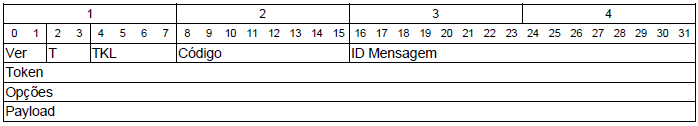
\includegraphics[width=0.8\textwidth]{imagens/coap_header.png}
\caption{Datagrama CoAP~\cite{shelby2014constrained}.
\label{fig:coap_header}}
\end{figure}
\FloatBarrier

Os campos que constituem o cabeçalho do datagrama são definidos pelo RFC 7252~\cite{shelby2014constrained} como:

\begin{itemize}
	\item \textbf{Versão (Ver)}: Inteiro não assinado de dois \textit{bits} que indica o número da correspondente versão do CoAP;
	\item \textbf{Tipo (T)}: Inteiro não assinado de dois \textit{bits} que indica se a mensagem é do tipo \textit{Confirmable} (0), \textit{Non-confirmable} (1), \textit{Acknowledgement} (2) ou \textit{Reset} (3);
	\item \textbf{Tamanho do \textit{token} (TKL)}: Inteiro não assinado de quatro \textit{bits} que indica o tamanho variável do \textit{token} para até 8 \textit{bytes}. Tamanhos de 9 a 15 \textit{bytes} são reservados e não devem ser enviados;
	\item \textbf{Código}: Inteiro não assinado de 8 \textit{bits} que caracteriza o tipo da mensagem, que pode ser um método de requisição (Tabela~\ref{tab:coap_met}) ou um código de resposta (Tabela~\ref{tab:coap_rep})   
\end{itemize}

\begin{table}[!ht]
	\centering\tiny{
	\caption{Códigos dos métodos CoAP~\cite{shelby2014constrained} \label{tab:coap_met}}
	\begin{tabular}{|c|c|}
		\hline
		\textbf{Código} & \textbf{Nome} \\ \hline
		0.01       &      GET      \\ \hline
		0.02       &     POST      \\ \hline
		0.03       &      PUT      \\ \hline
		0.04       &    DELETE     \\ \hline
	\end{tabular}
}
\end{table}

O cabeçalho é seguido de um \textit{token} utilizado para relacionar requisições e respostas. Ele é gerado pelo cliente e transportado junto da requisição. O \textit{token} deve então ser transmitido na resposta correspondente pelo servidor.

\begin{table}
	\centering\tiny{
	\caption{Códigos de resposta CoAP~\cite{shelby2014constrained}  \label{tab:coap_rep}}
	\begin{tabular}{|c|c|}
		\hline 
		\textbf{Código} & \textbf{Nome} \\ 
		\hline 
		2.01 & Criado \\ 
		\hline 
		2.02 & Deletado \\ 
		\hline 
		2.03 & Válido \\ 
		\hline 
		2.04 & Alterado \\ 
		\hline 
		2.05 & Conteúdo \\ 
		\hline 
		4.00 & \textit{Bad Request} \\ 
		\hline 
		4.01 & Não autorizado \\ 
		\hline 
		4.02 & \textit{Bad Option} \\ 
		\hline 
		4.03 & Proibido \\ 
		\hline 
		4.04 & Não encontrado \\ 
		\hline 
		4.05 & Método não permitido \\ 
		\hline 
		4.06 & Inaceitável \\ 
		\hline 
		4.12 & Precondição falhou \\ 
		\hline 
		4.13 & Entidade de requisição muito grande \\ 
		\hline 
		4.15 & \textit{Context-format} não suportado \\ 
		\hline 
		5.00 & Erro interno no servidor \\ 
		\hline 
		5.01 & Não implementado \\ 
		\hline 
		5.02 & \textit{Bad Gateway} \\ 
		\hline 
		5.03 & Serviço indisponível \\ 
		\hline 
		5.04 & \textit{Gateway timeout} \\ 
		\hline 
		5.05 & \textit{Proxing} não suportado \\ 
		\hline 
	\end{tabular} 
}
\end{table}
 \FloatBarrier
 
\subsection{MQTT}\label{sec:mqtt}

Criado em meados de 1999 por Andy Stanford-Clark (IBM) e Arlen Nipper (\textit{Eurotech}), o MQTT foi padronizado em 2014 pela \textit{Organization for the Advancement of Structured Information Standards} (OASIS) e encontra-se na versão 3.1.1~\cite{mqttv3.1.1}.

Com um cabeçalho fixo de apenas 2 \textit{bytes} e utilizando a estratégia publicação/assinatura para troca de mensagens, o MQTT é ideal para ambientes em IoT e demais contextos que exigem comunicação \textit{Machine-to-Machine} (M2M), onde  dispositivos com baixa capacidade computacional são inseridos em redes com latência, baixa largura de banda e alta taxa de perda de pacotes~\cite{mqttv3.1.1}.

O MQTT foi projetado para ser fácil de implementar, sendo que, deve ser usado juntamente com os protocolos TCP/IP nas camadas de transporte e rede, respectivamente, ou sobre outros protocolos que forneçam ordenação, comunicação sem perdas e conexões bidirecionais~\cite{mqttv3.1.1}. Estas características incluem:

\begin{itemize}
	\item Uso do padrão publicação/assinatura, provendo distribuição de mensagem um-para-muitos e dissociação das aplicações (Figura);
	\item Transporte de mensagens não influenciado pelo conteúdo do \textit{payload}.
	\item Entrega de mensagem com três níveis de \textit{Quality of Service} (QoS): "\textit{At most once}" (No máximo uma vez); "\textit{At least once}" (Ao menos uma vez); e "\textit{Exactly once}" (Exatamente uma vez) (Seção~\ref{sec:qos}).
	\item  Baixa sobrecarga de transporte e trocas de protocolo minimizadas, visando reduzir o tráfego na rede.
	\item Notificação às partes interessadas em caso de desconexões inesperadas.
\end{itemize} 

Para realizar a comunicação sobre a estratégia publicação/assinatura (do inglês, \textit{publish/subscriber}), o MQTT deve implementar um servidor próprio, chamado de \textit{broker}, que serve como intermediador para troca de mensagens entre os dispositivos.

\begin{figure}[ht]
	\centering
	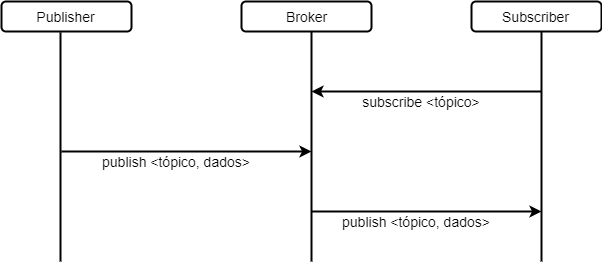
\includegraphics[width=0.8\textwidth]{imagens/mqtt_broker.png}
	\caption{Exemplo de comunicação MQTT sobre a estratégia publicação/assinatura (\textit{publish/subscribe}).
		\label{fig:mqtt_broker}}
\end{figure}
\FloatBarrier

Quando um dispositivo que atua como cliente deseja enviar uma mensagem para um ou mais clientes, o mesmo deve publicar um pacote de controle PUBLISH contendo os dados e um tópico. O servidor recebe o pacote PUBLISH, que é direcionado para os clientes previamente assinados no tópico correspondente. Os clientes que desejam receber as mensagens de um determinado tópico devem enviar um pacote SUBSCRIBE para o servidor com o tópico pretendido. Confirmada a assinatura, ele está apto a receber as mensagens publicadas no respectivo tópico, como ilustrado na figura~\ref{fig:mqtt_broker}.

Os pacotes de controle dos tipos  PUBLISH e SUBSCRIBE são apenas 2 dos 14 que podem ser usados durante a comunicação com o MQTT. Alguns podem ser usados em qualquer troca de mensagens, enquanto que outros dependem do nível de QoS das publicações ou de operações específicas para serem utilizados ou não.

A estrutura dos pacotes de controle, seus valores e tipos são descritas a seguir, e posteriormente o comportamento operacional do protocolo é abordado em relação ao níveo de QoS das publicações.

\subsubsection*{Pacotes de Controle} \label{sec:mqtt_format}

Um pacote de controle é um conjunto estruturado de \textit{bits} que contêm alguma informação que é emitida por meio de uma conexão de rede. Sendo que, a conexão de rede deve ser  providenciada por algum protocolo da camada de transporte.

Os pacotes MQTT podem ter até 3 elementos em sua estrutura, como mostra a Figura~\ref{fig:mqtt_format}. O primeiro destes é o cabeçalho fixo, presente em todos os pacotes, que pode ser seguido de um cabeçalho variável e um \textit{Payload}, ambos presentes em alguns tipos de pacotes, mas não em todos.

\begin{figure}[ht]
	\centering
	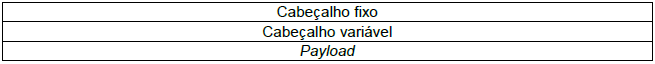
\includegraphics[width=0.8\textwidth]{imagens/mqtt_format.png}
	\caption{Estrutura de um pacote MQTT~\cite{mqttv3.1.1}.
		\label{fig:mqtt_format}}
\end{figure}
\FloatBarrier

O cabeçalho fixo possui 2 \textit{bytes}. Os \textit{bits} 7, 6, 5 e 4 do \textit{byte} 1, são usados para definir qual tipo de pacote será transmitido, enquanto que os \textit{bits} 3, 2, 1 e 0 são marcadores específicos para cada tipo de pacote, como ilustrado na Figura~\ref{fig:mqtt_pacFormat}. O \textit{byte} 2 corresponde ao campo de Largura Restante, que indica o número de \textit{bytes} restantes no pacote, incluindo dados do cabeçalho variável e do \textit{payload}.

\begin{figure}[ht]
	\centering
	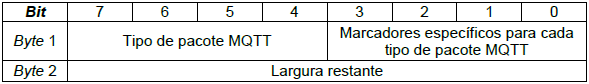
\includegraphics[width=0.8\textwidth]{imagens/mqtt_pacFormat.png}
	\caption{Formato do cabeçalho fixo MQTT~\cite{mqttv3.1.1}.
		\label{fig:mqtt_pacFormat}}
\end{figure}
\FloatBarrier

Com exceção do pacote PUBLISH, que pode ter seus marcadores definidos de variadas formas, todos os outros tipos de pacotes têm seus marcadores fixos, definidos de forma reservada. Nos pacotes PUBREL, SUBSCRIBE e UNSUBSCRIBE, os \textit{bits} 3, 2, 1 e 0 são fixados como 0, 0, 1 e 0, respectivamente, enquanto que nos outros (exceto PUBLISH), os 4 \textit{bits} devem ter valor 0.

O pacote PUBLISH conta com 3 marcadores específicos que abrangem os \textit{bits} 3, 2, 1 e 0 do cabeçalho fixo. A Figura~\ref{fig:mqtt_pubFormat} apresenta detalhes de seu formato, no qual o \textit{bit} 3 representa o marcador DUP, seguido de um indicador de nível de QoS envolvendo os \textit{bits} 2 e 1, e do sinalizador RETAIN, determinado pelo bit 0. A definição dos marcadores pode ser conferida nos tópicos abaixo:

\begin{itemize}
	\item \textbf{DUP}: Quando tem valor 0, o marcador DUP indica que essa é a primeira vez que o Cliente ou Servidor tentam enviar o pacote PUBLISH referido. Se o valor for 1, então aponta que o pacote teve que ser reenviado após uma tentativa prévia.
	\item \textbf{QoS}: Define o nível de QoS para o envio do pacote, os \textit{bits} podem assumir os seguintes valores: 0 e 0 (\textit{At most once}); 0 e 1 (\textit{At least once}); 1 e 0 (\textit{Exactly once}); e 1 e 1, que é reservado e não deve ser usado.
	\item \textbf{RETAIN}: quando um cliente envia uma mensagem PUBLISH ao servidor com este marcador ativado (RETAIN = 1), ela deve ser retida no servidor mesmo depois de ser entregue aos assinantes. No evento de uma
	nova subscrição a um tópico, a última mensagem retida para este tópico deve ser enviada para o
	novo assinante caso este marcador esteja ativado.
\end{itemize}

\begin{figure}[ht]
	\centering
	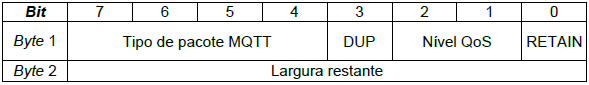
\includegraphics[width=0.8\textwidth]{imagens/mqtt_pubFormat.png}
	\caption{Formato do cabeçalho fixo de um pacote PUBLISH~\cite{mqttv3.1.1}.
		\label{fig:mqtt_pubFormat}}
\end{figure}
\FloatBarrier

Após o cabeçalho fixo, o pacote MQTT pode conter um cabeçalho variável, cujo conteúdo varia dependendo do tipo de pacote. O conteúdo mais comum é o Identificador de Pacote, que consiste na alocação de 2 \textit{bytes} para designar um valor único de identificação do pacote enquanto seu fluxo de entrega está em andamento.

O terceiro e último elemento de um pacote  MQTT é o \textit{payload}. Presente nos pacotes dos tipos CONNECT, PUBLISH (opcional), SUBSCRIBE, SUBACK e UNSUBSCRIBE, o conteúdo do \textit{payload} varia entre cada tipo de pacote. Em um pacote PUBLISH, por exemplo, o \textit{payload} contém a mensagem enviada pela aplicação.

A Tabela~\ref{tab:mqtt_packets} cita todos os 14 tipos de pacotes de controle, seus valores decimais, a direção de seu fluxo entre o Cliente (C) e o Servidor (S), seguidos de uma breve descrição.

\begin{table}[!ht]
	\centering\tiny{
		\caption{Pacotes de controle MQTT~\cite{mqttv3.1.1}} \label{tab:mqtt_packets}}
\begin{tabular}{|l|c|c|l|}
	\hline 
	\textbf{Nome} & \textbf{Valor} & \textbf{Direção de fluxo} & Descrição \\ 
	\hline 
	Reservado & 0 & Proibido & Reservado \\ 
	\hline 
	CONNECT & 1 & C $\rightarrow$ S & Requisição do cliente para conexão com o Servidor \\ 
	\hline 
	CONNACK & 2 & S $\rightarrow$ C & Confirmação de conexão. Resposta a um CONNECT \\ 
	\hline 
	PUBLISH & 3 & C $\rightarrow$ S ou S $\rightarrow$ C & Publicar mensagem \\ 
	\hline 
	PUBACK & 4 & C $\rightarrow$ S ou S $\rightarrow$ C & Confirmação de publicaçã. Resposta a um PUBLISH (QoS 1) \\ 
	\hline 
	PUBREC & 5 & C $\rightarrow$ S ou S $\rightarrow$ C & Publicação recebida (entrega assegurada 1). Resposta a um PUBLISH (QoS 2) \\ 
	\hline 
	PUBREL & 6 & C $\rightarrow$ S ou S $\rightarrow$ C & Publicação liberada (entrega assegurada 2). Resposta a um PUBREC (QoS 2) \\ 
	\hline 
	PUBCOMP & 7 & C $\rightarrow$ S ou S $\rightarrow$ C & Publicação completa (entrega assegurada 3). Resposta a um PUBREL (QoS 2) \\ 
	\hline 
	SUBSCRIBE & 8 & C $\rightarrow$ S & Requisição de assinatura de um Cliente \\ 
	\hline 
	SUBACK & 9 & S $\rightarrow$ C & Confirmação da assinatura. Resposta a um SUBSCRIBE \\ 
	\hline 
	UNSUBSCRIBE & 10 & C $\rightarrow$ S & Requisição para cancelar assinatura \\ 
	\hline 
	UNSUBACK & 11 & S $\rightarrow$ C & Confirmação de cancelamento de assinatura. Resposta a um UNSUBSCRIBE \\ 
	\hline 
	PINGREQ & 12 & C $\rightarrow$ S & Requisição de \textit{PING} \\ 
	\hline 
	PINGRESP & 13 & S $\rightarrow$ C & Resposta \textit{PING} \\ 
	\hline 
	DISCONNECT & 14 & C $\rightarrow$ S & Cliente está disconectando \\ 
	\hline 
	Reservado & 15 & Proibido & Reservado \\ 
	\hline 
\end{tabular} 
\end{table} 

\subsection{Níveis de \textit{Quality of Service} (QoS) do MQTT} \label{sec:qos}

O MQTT realiza a entrega das mensagens de acordo com os níveis de QoS definidos. O protocolo de entrega é simétrico, nas descrições e exemplos mostrados nesta seção, o Cliente (C) e o Servidor (S) podem assumir os papéis tanto de expedidor quanto de receptor. 

Além disso, a entrega de cada mensagem é concebida por um único expedidor e um único recebedor, pois quando o Servidor entrega uma mensagem para mais de um Cliente, cada Cliente é tratado independentemente.

Ademais, os diagramas de fluxo exibidos nesta seção são considerados exemplos de possíveis implementações.

\subsubsection*{QoS 0: \textit{At most once}}

Com a regra "\textit{At most once}" (No máximo uma vez), a entrega da mensagem depende das capacidades da rede subjacente. Não há resposta por parte do recebedor e nem reenvio por parte do expedidor, logo, a mensagem é recebida uma ou nenhuma vez.

A declaração normativa MQTT-4.3.1-1~\cite{mqttv3.1.1} define apenas uma ação que deve ser obrigatoriamente cumprida:
\begin{itemize}
	\item O expedidor deve enviar um pacote PUBLISH com QoS=0 e DUP=0.
\end{itemize}

Em caso de entrega concluída, o recebedor aceita a posse da mensagem (Figura~\ref{fig:mqtt_qos0}).

\begin{figure}[ht]
	\centering
	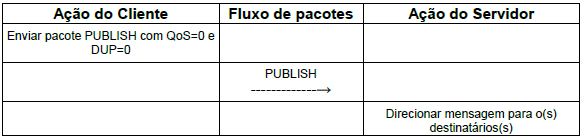
\includegraphics[width=0.9\textwidth]{imagens/mqtt_qos0.png}
	\caption{Exemplo de diagrama de fluxo para entrega com QoS 0~\cite{mqttv3.1.1}.
		\label{fig:mqtt_qos0}}
\end{figure}
\FloatBarrier

\subsubsection*{QoS 1: \textit{At least once}}

Este nível de QoS garante que a mensagem será entregue para o recebedor ao menos uma vez. Um pacote PUBLISH com QoS=1 possui um Identificador de Pacote em seu cabeçalho variável e sua entrega é confirmada com um pacote PUBACK.

Segundo a declaração normativa MQTT-4.3.2-1~\cite{mqttv3.1.1}, na entrega com  QoS 1, o expedidor deve:
\begin{itemize}
	\item Atribuir um Identificador de Pacote não usado sempre que haver uma nova mensagem a ser publicada;
	\item Enviar um pacote PUBLISH com QoS=1 e DUP=0 contendo este Identificador de Pacote;
	\item Tratar o pacote PUBLISH como "não confirmado" até que tenha recebido o correspondente pacote PUBACK do recebedor. 
\end{itemize}

O Identificador de Pacote torna-se disponível para uso novamente logo após o expedidor receber o pacote PUBACK.

Enquanto isso, a afirmação MQTT-4.3.2-2 define que o recebedor deve:
\begin{itemize}
	\item Responder com um pacote PUBLISH contendo o Identificador de Pacote do pacote PUBLISH correspondente, aceitando assim a posse da mensagem;
	\item Assim que enviar um pacote PUBACK, qualquer pacote PUBLISH recebido que possua o mesmo Identificador de Pacote deve ser tratado como uma nova publicação, independentemente do valor do marcador DUP.
\end{itemize}

\begin{figure}[ht]
	\centering
	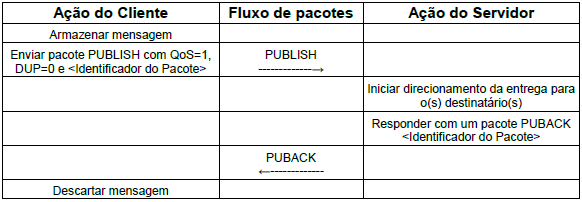
\includegraphics[width=0.9\textwidth]{imagens/mqtt_qos1.png}
	\caption{Exemplo de diagrama de fluxo para entrega com QoS 1~\cite{mqttv3.1.1}.
		\label{fig:mqtt_qos1}}
\end{figure}
\FloatBarrier

\subsubsection*{QoS 2: \textit{Exactly once}}

Este é o último nível de QoS, ideal para ser usado quando nenhuma perda ou duplicação de mensagens deve ser aceita. Assim como no QoS 1, suas mensagens também devem possuir um Identificador de Pacote atrelado ao seu cabeçalho variável.

A especificação do protocolo define um processo de duas etapas para confirmação de recepção das mensagens PUBLISH. Desta forma, o MQTT-4.3.3-1 determina que o expedidor deve:
\begin{itemize}
	\item Atribuir um Identificador de Pacote não usado quando houver uma nova mensagem a ser publicada;
	\item Enviar um pacote PUBLISH com QoS=2 e DUP=0 contendo este Identificador de Pacote;
	\item Tratar o pacote PUBLISH como "não confirmado" até que tenha recebido o respectivo pacote PUBREL do recebedor;
	\item Enviar um pacote PUBREL assim que receber o pacote PUBREC do recebedor. Sendo que, este pacote PUBREL deve conter o mesmo Identificador de Pacote do pacote PUBLISH original;
	\item Tratar o pacote PUBREL como "não confirmado" até que receba o pacote PUBCOMP correspondente do recebedor;
	\item Não deve reenviar o pacote PUBLISH, uma vez que seu respectivo pacote PUBREL tenha sido enviado.
\end{itemize}

O Identificador de Pacote torna-se disponível para reuso logo após o expedidor receber o pacote PUBCOMP.

No entretanto, o MQTT-4.3.3-2~\cite{mqttv3.1.1} define que o recebedor deve:
\begin{itemize}
	\item Responder com um pacote PUBREC contendo o Identificador de Pacote do pacote PUBLISH recebido, aceitando assim a posse da mensagem;
	\item Enquanto não receber o pacote PUBREL correspondente, o recebedor deve confirmar qualquer pacote PUBLISH subsequente que tenha o mesmo Identificador de Pacote por meio do envio de um PUBREC. Nesse caso, o método não pode causar duplicação de mensagens;
	\item Responder um pacote PUBREL por meio do envio de um pacote PUBCOMP contendo o mesmo Identificador de Pacote;
	\item Depois que enviar um PUBCOMP, o recebedor deve tratar qualquer pacote PUBLISH recebido que tenha o mesmo Identificador de Pacote como uma nova publicação.
\end{itemize}

\begin{figure}[ht]
	\centering
	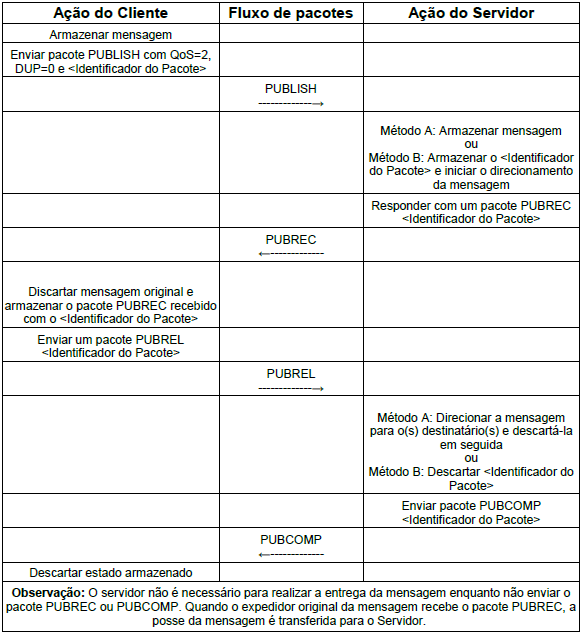
\includegraphics[width=0.9\textwidth]{imagens/mqtt_qos2.png}
	\caption{Exemplo de diagrama de fluxo para entrega com QoS 2~\cite{mqttv3.1.1}.
		\label{fig:mqtt_qos2}}
\end{figure}
\FloatBarrier

No caso ilustrado na Figura~\ref{fig:mqtt_qos2}, a escolha dos métodos A ou B por parte do recebedor fica a critério da implementação. Desde que seja escolhido apenas um dos métodos, as garantias presentes no QoS 2 não serão afetadas.

\subsection{Comparação com outros protocolos}\label{sec:protocols}

Diversos protocolo de aplicação são propostos para soluções em IoT, cada um com seus aspectos específicos para prover comunicação.

A escolha do protocolo deve levar em conta fatores como: capacidade de processamento e armazenamento dos dispositivos; limitações do ambiente; e tipo de comunicação (\textit{Machine-to-Machine}, \textit{Machine-to-Server} ou \textit{Server-to-Server})~\cite{al2015toward}.

Além dos protocolos HTTP, CoAP e MQTT apresentados anteriormente, a Figura~\ref{fig:tabela_protocolos} cita também outros protocolos de destaque no cenário de IoT e suas principais características. 

\begin{figure}[ht]
	\centering
	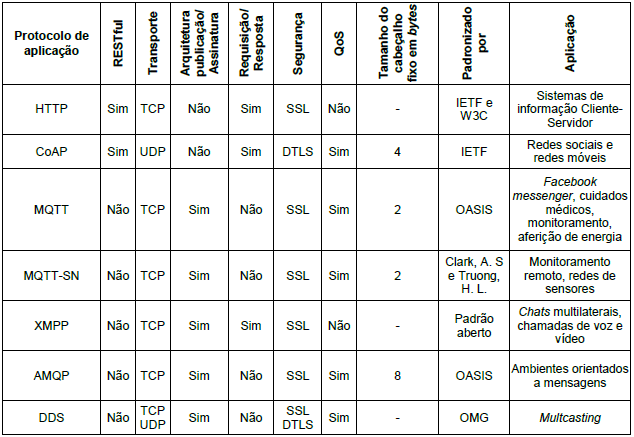
\includegraphics[width=1\textwidth]{imagens/tabela_protocolos.png}
	\caption{Características e propriedades dos protocolos de aplicação em IoT~\cite{sankarinternet}, adaptado pelo autor.
		\label{fig:tabela_protocolos}}
\end{figure}
\FloatBarrier

O protocolo MQTT-SN é uma adaptação do MQTT voltada para redes de sensores, pois é mais leva e exige ainda menos recursos em relação ao MQTT~\cite{stanford2013mqtt}.

Utilizando uma arquitetura baseada em um \textit{broker}, o DDS (\textit{Data Distribution Service})~\cite{dds2015specifi} é semelhante ao MQTT. Porém, o DDS mostra-se mais adequado para serviços. Uma das principais diferenças está no suporte para \textit{Qualities os Service}, enquanto o MQTT detêm 3 níveis de QoS, o DDS opera com 23, além do suporte a implementação com UDP e DTLS.

Portando aplicabilidades distintas, o AMQP~\cite{amqp2012oasis} e o XMPP~\cite{xmpp2011extensible}, mostram-se ideais para ambientes orientados a mensagens e \textit{chats} multilaterais de mensagem, voz e vídeo, respectivamente.

Ao analisar as particularidades de cada protocolo, percebe-se o caráter mais abrangente do CoAP e do MQTT, enquanto que os demais são projetados para ambientes mais específicos, o que não impede que uma aplicação complexa possa empregar diferentes protocolos em diferentes contextos.   

\section{Contratos}

Desde os princípios da sociedade moderna, os compromissos, normas, regras e padrões regem o relacionamento entre as pessoas~\cite{mura2016}. A origem etimológica do vocábulo contrato conduz ao vínculo jurídico das vontades com vistas a um objeto específico, sendo um acordo e vontades criador de direitos e obrigações entre as partes envolvidas~\cite{miranda2008teoria}. Um contrato reflete a vontade entre dois ou mais indivíduos no intuito de adquirir, resguardar, modificar, transferir ou extinguir direitos, garantindo a vontade dos mesmos sobre um determinado assunto~\cite{mura2016, miranda2008teoria}. Segundo~\cite{gomes2007contratos}, contrato é o acordo jurídico bilateral, ou plurilateral, que atribui as partes a responsabilidade de observância de conduta idônea à satisfação dos interesses que regularam.

Os contratos podem ser classificados conforme a atribuição de responsabilidades. Contratos unilaterais são aqueles no qual um indivíduo assume responsabilidades, enquanto que nos contratos bilaterais, dois indivíduos assumem responsabilidades. Já em contratos multilaterais, três ou mais indivíduos assumem responsabilidades~\cite{miranda2008teoria}.

A negociação de contratos entre os indivíduos pode resultar na combinação de cláusulas de interesse de cada um. Essa combinação pode acarretar em diversos problemas, tal como os conflitos normativos~\cite{ausin2005logica}, em que ocorrem uma ou mais contradições entre as normas~\cite{bobbio1999teoria}. Um conflito faz com que o contrato torne-se inválido, visto que não há como satisfazê-lo sem violar ou desconsiderar alguma das normas estabelecidas~\cite{ausin2005logica}.

A quebra de um contrato ocorre mediante a violação de alguma cláusula por parte de um ou mais indivíduos. Posto isto, pode ser interessante para as partes envolvidas no contrato, ter conhecimento de quais indivíduos estão relacionados direta ou indiretamente com a violação. Portanto, no processo de monitoramento da execução de um contrato as partes envolvidas em cada ação a ser tomada devem ser levadas em conta, possibilitando a identificação dos envolvidos numa quebra contratual. 

\subsection{Contratos eletrônicos}

Um contrato eletrônico ou \textit{"e-Contract"} é um meio para representação digital dos contratos convencionais, utilizados para firmar acordos entre pessoas ou entidades. Desta forma, a tecnologia é utilizada como aliada na solução de problemas encontrados neste contexto. Assim como em contratos convencionais, um contrato eletrônico engloba as obrigações de cada participante, atividades exercidas e responsabilidades definidas para cada um dos indivíduos para satisfazer os termos e condições do contrato estabelecido~\cite{xu2004monitoring}.

São diversas as áreas de aplicação dos contratos eletrônicos. Em meios legais, contratos físicos são convertidos ou substituídos para o meio eletrônico. Técnicas de contratação eletrônica em sistemas, lógicas de negócio ou integração de serviços também podem ser utilizadas. A contratação eletrônica legal visa a criação de um documento contratual que busca expressão a intenção das partes envolvidas~\cite{xu2004monitoring}. As ferramentas para contratação eletrônica buscam informar as partes acerca dos efeitos das disposições contratuais, auxiliar na verificação e execução do contrato, assim como monitorar sua execução~\cite{mura2016}.

A lei considera contratos como um conjunto de obrigações e o mesmo se aplica ao meio eletrônico. O contrato eletrônico tem como aliado o apoio computacional e automatizado, que permite verificar, controlar e monitorar de forma mais eficiente~\cite{mura2016}.

\subsubsection*{Topologia dos contratos eletrônicos}

A topologia de um contrato eletrônico pode ser definida de acordo com o número de participantes envolvidos, bem como a complexidade das relações de direitos e deveres entre os mesmos~\cite{angelov2001b2b}. 

Um contrato bilateral tem como característica principal o acordo entre no máximo dois indivíduos, que estabelecem um contrato com obrigações de ambos. O contrato em cadeia inclui a participação de vários indivíduos, porém, em forma de sub-contratos, dos quais vários acordos bilaterais são estabelecidos. Já no contrato multilateral, os vários indivíduos envolvidos podem interagir entre si, de forma a causar dependências mais complexas do que no modelo em cadeia, pois um indivíduo pode ter cláusulas e dependências que envolvem responsabilidades por parte de outros indivíduos~\cite{mura2016}.

Contratos complexos podem ser divididos em sub-contratos bilaterais para facilitar sua execução. Porém, essa divisão não pode ser realizada sem a perda de informações importantes em contratos multilaterais~\cite{xu2004multi}. Portanto, um conjunto de contratos bilaterais não é capaz de expressar a complexidade do relacionamento entre os indivíduos de um contrato multilateral, visto que a perda de informações e a diminuição da expressividade das normas do contrato é um fator iminente~\cite{mura2016}.  

\subsection{Verificação de contratos eletrônicos}

Variadas pesquisas já foram realizadas no âmbito dos contratos eletrônicos, especialmente na verificação dos mesmos. Além de acelerar sua escrita, a automatização de um contrato permite que suas propriedades sejam formalmente verificadas~\cite{fenech2008conflict}. Algumas das técnicas e abordagens mais comuns em contratos eletrônicos são:

\begin{itemize}
	\item \textbf{Negociação:} Cenário em que pelo menos dois indivíduos propõem soluções e contrapostas de seu interesse, visando alcançar um acordo aceitável por ambas as partes envolvidas. Este processo é realizado em contratos bilaterais e multilaterais é pode envolver ou não o uso de mediadores~\cite{bosse2008automated}.
	\item \textbf{Detecção de conflitos:} A detecção de conflitos~\cite{xu2004monitoring} visa a detecção e eliminação de conflitos normativos de um contrato, pois esta situação invalida um contrato, induzindo a uma violação~\cite{bobbio1999teoria}.
	\item \textbf{Assinatura:} De forma geral, a assinatura de um contrato digital gera mais complicações do que no modo convencional. Isso deve-se ao fato de que nenhum indivíduo quer ser o primeiro a assinar o contrato, pois um indivíduo pode recusar-se a assiná-lo após obter a assinatura e o contrato do primeiro indivíduo, o que pode causar uma vantagem indesejada para um dos envolvidos~\cite{chadha2006formal, kordy2012constructing}.
	\item \textbf{Monitoramento:} Durante a execução do contrato, o monitoramento tem a função de verificar se as cláusulas são respeitadas pelos participantes. Um contrato é violado quando alguma cláusula é ignorada por um dos participantes. Tornando as transações e relacionamentos entre os indivíduos mais confiáveis, flexíveis, eficientes e aceitáveis, é possível manter os benefícios entre todos os indivíduos na presença de violações~\cite{xu2004monitoring}. Sendo assim, um sistema de monitoramento de contratos precisa saber quais ações são aceitáveis ou esperadas de um indivíduo, assim como identificar o responsável por uma violação, caso ocorra~\cite{xu2004monitoring}.
\end{itemize}  

\section{Representação formal de sistemas}

Com a utilização de formalismos para expressar contratos alguns problemas normalmente encontrados em contratos convencionais são evitados, como inconsistências e ambiguidades. Portanto, a definição de um formalismo adequado faz parte do processo de verificação de contratos eletrônicos~\cite{fenech2008conflict}. A seguir são descritas proposicional e temporal, normalmente utilizadas para representar sistemas e propriedades.

\subsection{Lógica proposicional}
   
Geralmente, qualquer cálculo matemático é criado com a intenção de representar um certo domínio de objetos formais, normalmente com o objetivo de facilitar as computações e inferências que precisam ser realizadas sobre esta representação~\cite{bedregal2002logica}. Em lógica e matemática, uma lógica proposicional é um sistema formal em que fórmulas representam proposições formadas por proposições atômicas usando conectivos lógicos e um sistema de regras de derivação, desta forma, as fórmulas podem ser consideradas como teoremas do sistema formal~\cite{bedregal2002logica}.

A lógica proposicional tem como objetivo modelar o raciocínio humano, partindo de proposições, como frases declarativas~\cite{bedregal2002logica}. Por exemplo, considerando-se a frase "1 mais 1 é igual a 10", ou simbolicamente, "1 + 1 = 10". Esta frase pode ser considerada uma asserção declarativa, visto que afirma ou nega um fato, portanto representa uma proposição com valor verdadeiro ou falso. Neste caso, a proposição é verdadeira, num sistema numérico de base 2, ou falsa, caso o sistema seja decimal. Portanto, a lógica proposicional estuda formas de raciocínio sobre afirmações que podem ser verdadeiras ou falsas, além de definir meios para construção de demonstrações que provem que uma determinada conclusão é verdadeira num certo contexto, levando em conta um conjunto de hipóteses~\cite{bedregal2002logica}.

A sintaxe do cálculo proposicional é definida por um alfabeto constituído por~\cite{souza2017logica}:
\begin{itemize}
	\item \textbf{Símbolos de pontuação:} $($, $)$;
	\item \textbf{Símbolos de verdade:} $true~(\top)$, $false~(\perp)$;
	\item \textbf{Símbolos proposicionais:} $P,~Q,~R,~S,~P_{1},~Q_{1},~R_{1},~S_{1},~... $;
	\item \textbf{Conectivos proposicionais:} $\neg,~\wedge,~\vee,~\rightarrow,~\leftrightarrow$.
\end{itemize}

Para um melhor entendimento, a Tabela~\ref{tab:prop_conec} apresenta algumas formas de leitura para linguagem natural atribuídas aos conectivos proposicionais.

\begin{table}[!ht]
	\centering\tiny{
		\caption{Leituras dos conectivos proposicionais para a linguagem natural~\cite{abe2002introduccao}. \label{tab:prop_conec}}
\begin{tabular}{|l|c|l|}
	\hline 
	\textbf{Conectivo} & \textbf{Exemplo} & \textbf{Leitura} \\ 
	\hline 
	Negação $\neg$ & $\neg A$ & Não $A$; \\ & & Não se dá que $A$; \\ & & Não é verdade que $A$. \\ 
	\hline 
	Conjunção $\wedge$ & $A\wedge B$ & $A$ e $B$; \\ & & $A$, mas $B$; \\ & & $A$, embora $B$; \\ & & $A$, assim como $B$. \\ 
	\hline 
	Disjunção $\vee$ & $A\vee B$ & $A$ ou $B$ ou ambos. \\ 
	\hline 
	Implicação $\rightarrow$ & $A\rightarrow B$ & se $A$, então $B$; \\ & & se $A$, isto significa que $B$; \\ & & tendo-se $A$, então $B$; \\ & & $A$ implica $B$; \\ & & $B$ é implicada por $A$. \\ 
	\hline 
	Bi-implicação $\leftrightarrow$ & $A\leftrightarrow B$ & $A$ se e somente se $B$; \\ & & $A$ quando e somente quando $B$; \\ & & $A$ equivale a $B$. \\ 
	\hline 
\end{tabular}   
	}
\end{table}

Um cálculo proposicional é um sistema formal $\mathcal{L} = (\mathcal{A},~\Omega,~\mathcal{Z},~\mathcal{I})$, em que $\mathcal{A}$ é um conjunto finito de símbolos proposicionais. Conhecidos também como fórmulas atômicas ou elementos terminais, os elementos de $\mathcal{A}$ são os mais básicos da linguagem formal $\mathcal{L}$, sintaticamente falando~\cite{bedregal2002logica}. No decorrer desta sessão, os elementos de $\mathcal{A}$ serão denotados como $P,~Q,~R,$ em diante.

O conjunto $\Omega$ compreende a coleção de símbolos de verdade e dos conectivos proposicionais, ou conectivos lógicos, e é dividido entre conjuntos distintos, de forma que $\Omega = \Omega_{0}\cup \Omega_{1} \cup ... \cup \Omega_{j} \cup ... \cup \Omega_{m}$. Nesta divisão, $\Omega_{j}$ é o conjunto dos símbolos de aridade $j$~\cite{bedregal2002logica}.

A linguagem, ou conjunto de fórmulas $\mathcal{L}$, é definida recursiva ou indutivamente pelas seguintes regras~\cite{bedregal2002logica, abe2002introduccao}:
\begin{itemize}
	\item Qualquer elemento do conjunto $\mathcal{A}$ é uma fórmula de $\mathcal{L}$;
	\item Se $P$ é uma fórmula, então $\neg P$, a negação de $P$, é uma fórmula;
	\item Se $P$ e $Q$ são fórmulas, então a disjunção dada por $P \vee Q$, é uma fórmula;
	\item Se $P$ e $Q$ são fórmulas, então a conjunção dada por $P \wedge Q$, é uma fórmula;
	\item Se $P$ e $Q$ são fórmulas, então a implicação dada por $P \rightarrow Q$, é uma fórmula, tal que $P$ é o antecedente, e $Q$, o consequente.
	\item se $P$ e $Q$ são fórmulas, então a bi-implicação dada por $P \leftrightarrow Q$, é uma fórmula.     
\end{itemize}

O conjunto $\mathcal{Z}$ é a coleção finita de regras de inferência~\cite{bedregal2002logica}. Já o conjunto $\mathcal{I}$ é a coleção finita de pontos iniciais, também chamados de axiomas~\cite{bedregal2002logica}.

As propriedades semânticas da Lógica Proposicional podem ser determinadas por meio uma Tabela-verdade, em que cada linha, exceto a primeira, representa uma valoração para cada sub-fórmula de uma dada fórmula em relação aos possíveis valores de suas proposições. Seguindo o princípio da bivalência, os valores para cada átomo da tabela possui favor verdadeiro (V) ou falso (F)~\cite{bedregal2002logica}.

A Tabela~\ref{tab:conectivos} demonstra as propriedades dos conectivos de negação, conjunção, disjunção, implicação e bi-implicação, respectivamente. O operador pode ser adicionado indefinidamente, mesmo que não haja necessidade, visto que $\neg \neg P \equiv P$ e $\neg \neg \neg P \equiv \neg P$. Nota-se que a conjunção entre duas fórmulas só é verdadeira quando ambas são verdadeiras, enquanto que, a disjunção entre duas fórmulas só é verdadeira quando ao menos uma delas é verdadeira. A implicação entre duas fórmulas só é falsa se a da esquerda (antecedente) for verdadeira e a da direita (consequente) for falta. Sendo assim, das propriedades descritas, a implicação é a única não comutativa, ou seja, a ordem das proposições envolvidas alteram seu resultado. Por fim, a bi-implicação, ou equivalência, entre duas fórmulas é verdadeira quando ambas são verdadeiras ou ambas são falsas.

\begin{table}[!ht]
	\centering\tiny{
		\caption{Tabela verdade dos conectivos proposicionais. \label{tab:conectivos}}
\begin{tabular}{|c|c|c|c|c|c|c|c|c|c|c|c|c|}
	\hline 
	\multicolumn{2}{|c|}{\textbf{Proposições}}  & \multicolumn{11}{c|}{\textbf{Conectivos proposicionais}} \\ 
	\hline
	\multicolumn{2}{|c|}{} 
	& \multicolumn{3}{c|}{\textbf{Negação} $\neg$} & \multicolumn{2}{c|}{\textbf{Conjunção} $\wedge$}  & \multicolumn{2}{c|}{\textbf{Disjunção} $\vee$}  & \multicolumn{2}{c|}{\textbf{Implicação} $\rightarrow$}  & \multicolumn{2}{c|}{\textbf{Bi-implicação} $\leftrightarrow$}   \\ 
	\hline 
	$~~\textbf{P}~~$ & $\textbf{Q}$ & $\neg P$ & $\neg \neg P$ & $\neg \neg \neg P$ & $P \wedge Q$ & $Q \wedge P$ & $P \vee Q$ & $Q \vee P$ & $P \rightarrow Q$ & $Q \rightarrow P$ & $P \leftrightarrow Q$ & $Q \leftrightarrow P$ \\ 
	\hline 
	V & V & F & V & F & V & V & V & V & V & V & V & V \\ 
	\hline 
	V & F & F & V & F & F & F & V & V & F & V & F & F \\ 
	\hline 
	F & V & V & F & V & F & F & V & V & V & F & F & F \\ 
	\hline 
	F & F & V & F & V & F & F & F & F & V & V & V & V \\ 
	\hline 
\end{tabular}   
	}
\end{table}

A construção de uma Tabela-verdade consiste em dois passos: primeiro é definida uma linha em que estão contidas as proposições presentes numa dada fórmula, assim como as sub-fórmulas, seguidas da própria fórmula; no segundo passo são preenchidas as linhas $l$, em que estão todos os possíveis valores que as proposições atômicas podem receber e os valores recebidos pelas fórmula a partir dos valores das proposições. O número de linhas é $l = n^{t}$, sendo $n$ o número de valores que o sistema permite (verdadeiro ou falso) e $t$, o número de proposições atômicas que a fórmula possui.

Dada a fórmula $((P \vee Q)\rightarrow (Q \wedge (Q \leftrightarrow P)))$, tem-se o conjunto de sub-fórmulas ${(Q \wedge (Q \leftrightarrow P)),~(Q \leftrightarrow P),~(P \vee Q), P, Q}$. Como há apenas duas proposições atômicas, $P$ e $Q$, então $t = 2$, logo, $l = 2^{2} = 4$. Baseado nisso, obtêm-se a valoração completa, exibida na Tabela~\ref{tab:conec_exe}.

Outra forma de se observar as propriedades semânticas das fórmulas proposicionais é por meio da construção de uma árvore de derivação, na qual a fórmula é deriva em suas sub-fórmulas repetidamente até que as "folhas" da árvores contenham apenas as proposições atômicas, como ilustrado na Figura~\ref{fig:ex_arvore}.

\begin{figure}[ht]
	\centering
	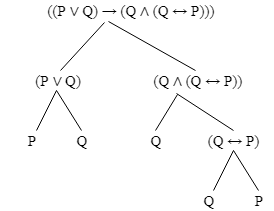
\includegraphics[width=0.4\textwidth]{imagens/ex_arvore.png}
	\caption{Árvore de derivação associada à fórmula $((P \vee Q)\rightarrow (Q \wedge (Q \leftrightarrow P)))$.
		\label{fig:ex_arvore}}
\end{figure}
\FloatBarrier

\begin{table}[!ht]
	\centering\tiny{
		\caption{Tabela verdade associada à fórmula $((P \vee Q)\rightarrow (Q \wedge (Q \leftrightarrow P)))$. \label{tab:conec_exe}}
\begin{tabular}{|c|c|c|c|c|c|}
	\hline 
	$\textbf{P}$ & $\textbf{Q}$ & $(P \vee Q)$ & $(Q \leftrightarrow P)$ & $(Q \wedge (Q \leftrightarrow P))$ & $((P \vee B) \rightarrow (Q \wedge (Q \leftrightarrow P)))$ \\ 
	\hline 
	V & V & V & V & V & V \\ 
	\hline 
	V & F & V & F & F & F \\ 
	\hline 
	F & V & V & F & F & F \\ 
	\hline 
	F & F & F & V & F & V \\ 
	\hline 
\end{tabular} 
}
\end{table}

A lógica proposicional é considerada um dos tipos mais simples de calculo lógico, podendo ser estendida de diversas formas. Com a adição de novas regras e definições, outras lógicas podem ser desenvolvidas, como, por exemplo, a lógica de primeira ordem~\cite{smullyan1995first},  as lógicas modais~\cite{chellas1980modal}, e a lógica temporal~\cite{pnueli1977temporal}.
   
\subsection{Lógica temporal}

A lógica temporal é um formalismo usado para descrever sequências de transações entre estados em sistemas reativos~\cite{clarke1999model}. Portanto, uma fórmula lógica temporal geralmente é avaliada sobre um sistema de transição que modela uma especificação~\cite{clarke1999model}, isto é, um modelo de \textit{Kripke}~\cite{kripke1959completeness}.

Na lógica temporal, o modelo é dado pela tupla $\mathcal{M} = (S, \rightarrow, L)$, em que $S$ é o conjunto de estados, $\rightarrow$ (ou $R$) $ \in S \times S$ é a relação de transição e $L \colon S \rightarrow 2^{AP}$ denota a função de rotulação dos estados com as proposições atômicas $AP$ verdadeiras no estado em que se encontram. 

Um exemplo de sistema de transição é apresentado na Figura~\ref{fig:temporal_grafo}, definido por:
\begin{itemize}
	\item $AP = \{p,q,r\}$
	\item $S = \{s_{0}, s_{1}, s_{2}\}$
	\item $\rightarrow = \{(s_{0}, s_{1}), (s_{1}, s_{0}), (s_{0}, s_{2}), (s_{1}, s_{2}), (s_{2}, s_{2})\}$
	\item $L(s_{0}) = \{p,q\}, L(s_{1}) = \{q, r\}, L(s_{2}) = \{r\}$
\end{itemize}

\begin{figure}[ht]
	\centering
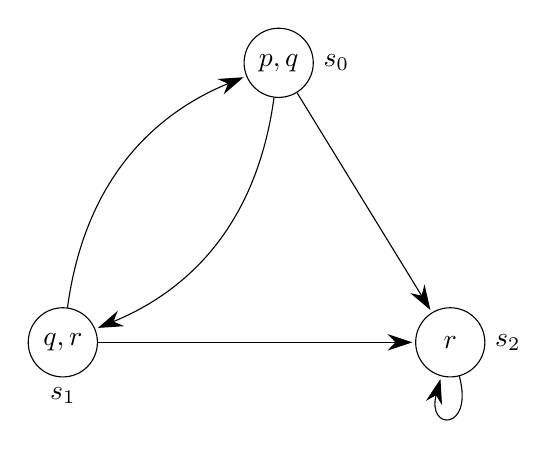
\begin{tikzpicture}[>={Stealth[width=6pt,length=9pt]}, accepting/.style={double distance = 2pt, outer sep = 1pt + \pgflinewidth}, shorten >=1pt, auto]
\draw (158.0pt, -70.0pt)node[state, label=right:$s_{0}$](0){$p,q$};
\draw (80.0pt, -171.0pt)node[state, label=below:$s_{1}$](1){$q,r$};
\draw (220.0pt, -171.0pt)node[state, label=right:$s_{2}$](2){$r$};
\path[->] (2) edge[loop below] node{}(2);
\path[->] (1) edge node{}(2);
\path[->] (0) edge node{}(2);
\path[->] (1) edge[bend left] node{}(0);
\path[->] (0) edge[bend left] node{}(1);
\end{tikzpicture}
\caption{Exemplo de um sistema de transição~\cite{huth2004logic}.
	\label{fig:temporal_grafo}}
\end{figure}
\FloatBarrier

Uma fórmula lógica temporal pode ser verdadeira ou falsa dependendo do modelo no qual é interpretada. O conjunto de estados representam a evolução do sistema ao longo do tempo e as fórmulas são avaliadas em cada estado do sistema. Portanto, a noção estática de verdade é substituída pela noção dinâmica de evolução dos estados do sistema ao longo do tempo~\cite{clarke1999model}.

A lógica temporal pode ser dos tipos linear ou ramificada. Na abordagem linear, o tempo é tratado como se cada momento tivesse apenas um único futuro possível, logo, as fórmulas são interpretadas como sequências lineares, ou caminhos. Já na abordagem ramificada, cada estado pode evoluir para uma ramificação de vários futuros possíveis, de acordo com a evolução do sistema, com uma representação em árvore~\cite{mura2016}.

\subsubsection{Lógica temporal linear}

Como dito acima, uma lógica temporal compreende a evolução de um sistema de transição de estados ao longo do tempo. Diante disso, a lógica temporal linear (ou LTL) possui conectivos que se referem ao futuro, e suas fórmulas são interpretadas sobre uma sequência de estados chamada de \textit{path} (caminho). Um \textit{path} é uma sequência finita não vazia denotada por $\pi = \langle \pi_{0}, \pi_{1}, \ldots, \pi_{n-1} \rangle$, em que os estados $\pi_{0}, \pi_{1}, \ldots, \pi_{n-1} \in S$ e $(\pi_{i}, \pi_{i-1}) \in R$ para todo $0 \leq i < n-1$. O tamanho de um \textit{path} é denotado por $|\pi|=\infty$. Um \textit{path} infinito é denotado por $\pi = \langle \pi_{0}, \pi_{1}, \pi_{3}, \ldots \rangle$ com tamanho $|\pi| = \infty$. Todo \textit{path} que não pode ser estendido é considerado maximal, logo, qualquer \textit{path} infinito é maximal~\cite{muller1999invited}.

A sintaxe de uma fórmula LTL é composta de proposições atômicas e gerada conforme segue:
\begin{equation}
\varphi ::= \top~|~\bot~|~p~|~\neg \varphi~|~\varphi \vee \varphi~|~\varphi \rightarrow \varphi~|~X\varphi~|~F\varphi~|~G\varphi~|~\varphi U \varphi'
\end{equation}

Assim como na lógica proposicional, os valores lógicos avaliados como verdadeiro e falso são representados pelos símbolos $\top$ e $\bot$, respectivamente, além dos operadores lógicos $\neg$, $wedge$, $\vee$ e $\rightarrow$, que também têm o mesmo significado. Já o símbolo $p$ representa um identificador das proposições, e os operadores $X$, $F$, $G$ e $U$, são usados para especificar situações temporais de uma fórmula. A expressão $X\varphi$ (após $\varphi$) indica que a proposição $\varphi$ é verdadeira no próximo estado. Já a expressão $F\varphi$ (afinal, $\varphi$) configura que em algum estado futuro da computação, $\varphi$ é verdadeira, enquanto que $G\varphi$ (sempre $\varphi$) indica que $\varphi$ é verdadeira em todos os estados do caminho de computação. Enfim, a expressão $\varphi U \varphi'$ ($\varphi$ até que $\varphi'$) significa que a proposição $\varphi$ deve ser verdadeira em todos os estados até que $\varphi$ seja verdadeira~\cite{mura2016, muller1999invited}. 

Uma fórmula $\alpha$ em LTL é satisfeita se existe um modelo $M$ e um \textit{path} $\pi$ tal que $\mathcal{M}, \pi \models \varphi$, ou seja, um modelo no qual o \textit{path} $\pi$ satisfaz a fórmula $\varphi$. Um \textit{path} é formado por uma sequência de estados $s$ e suas posições são indexadas partindo de $\pi_{1}$ até $\pi_{n}$, em que $n$ a quantidade de posições de $\pi$. Sendo $\pi$ um dado \textit{path} de $\mathcal{M}$, as relações de satisfação $\models$ e $\nvDash$ indicam se uma fórmula LTL é satisfeita ou não, respectivamente, por $\pi$~\cite{huth2004logic}, como exposto a seguir: 

\begin{figure}[ht]
	\centering
	\begin{align}
	&\pi \models \top \label{eq:l1} \\
	&\pi \nvDash \bot \label{eq:l2} \\
	&\pi \models p \Longleftrightarrow p \in L(\pi_{1}) \label{eq:l3} \\
	&\pi \models \neg \varphi \iff \pi \not \models \varphi \label{eq:l4} \\
	&\pi \models \varphi \wedge \varphi' \iff \pi \models \varphi \mbox{ e } \pi \models \varphi' \label{eq:l5}\\
	&\pi \models \varphi \vee \varphi' \iff \pi \models \varphi \mbox{ ou } \pi \models \varphi' \label{eq:l6}\\
	&\pi \models \varphi \to \varphi' \iff \pi \models \varphi \mbox{ sempre que } \pi \models \varphi' \label{eq:l7}\\
	&\pi \models X\varphi \iff \pi_2 \models \varphi \label{eq:l8}\\
	&\pi \models G\varphi \iff \forall i \geq 1 \mid \pi_i \models \varphi \label{eq:l9}\\
	&\pi \models F\varphi \iff \exists i \geq 1 \mid \pi_i \models \varphi \label{eq:l10}\\
	&\pi \models \varphi U \varphi' \iff \exists i \geq 1 \mid \pi_i \models \varphi' \mbox{ e } \forall j = 1 \wedge j < i \mid \pi_j \models \varphi \label{eq:l11}
	\end{align}
	\caption{Semântica da LTL.
		\label{fig:ltl_sem}}
\end{figure}
\FloatBarrier

As definições~\ref{eq:l1} e~\ref{eq:l2} da Figura~\ref{fig:ltl_sem} indicam as proposições verdadeiras e falsas, respectivamente. Na definição~\ref{eq:l3} é dito que a proposição $p$ só é válida se estiver no primeiro estado do \textit{path}. Nas proposições~\ref{eq:l4} a~\ref{eq:l7} são definidos os conectivos proposicionais da lógica proposicional. Em~\ref{eq:l8}, o operador $X$ denota que a fórmula $\varphi$ é satisfeita no próximo estado, no caso, a segunda posição do \textit{path}. As definições~\ref{eq:l9} e~\ref{eq:l10} representam os operadores $G$ e $F$ que apontam, respectivamente, que a fórmula $\varphi$ é verdadeira em todas ou em pelo menos uma posição de $\pi$. Por fim, a definição~\ref{eq:l11} representa o operador $U$, expressando que, para toda posição antecessora à $\pi_{i}$, a fórmula $\varphi$ é verdadeira, caso contrato, a proposição $\varphi'$ é verdadeira.

Diversas propriedades relevantes podem ser verificadas com fórmulas LTL, tais como, de segurança, no qual o sistema é livre de \textit{deadlocks}, e de progresso, em que toda requisição realizada é atendida~\cite{mura2016, huth2004logic}. ~\citeauthor{huth2004logic} descreve algumas propriedades que podem ser representadas em sistemas reais, considerando um sistema especificado com as proposições $ocupado$, $requisitado$, $iniciado$, $pronto$ e $habilitado$, como nos exemplos a seguir:

\begin{itemize}
	\item o sistema não pode ter $iniciado$ e ainda não estar $pronto$ para atender requisições: 
	\begin{equation}
	G\neg(iniciado\wedge\neg\;pronto)
	\end{equation} 
	\item em todo sistema, se é $requisitado$ algum recurso, o requisitante deve ser $respondido$:
	\begin{equation}
	G(requisitado \to F\;respondido)
	\end{equation}
	\item um processo é $habilitado$ infinitas vezes em todo o caminho de computação: 
	\begin{equation}
	GF\;habilitado 
	\end{equation}
	\item um elevador subindo para o segundo andar não muda sua direção quando houver passageiros que desejam ir para o quinto andar: 
	\begin{equation}
	G(andar2 \wedge subindo \wedge pressionadoBotao5 \to (subindo U andar5))
	\end{equation}
\end{itemize}

Os exemplos acima demonstram que a LTL é capaz de representar propriedades essenciais em sistemas de transição de estados. Porém, há propriedades que não podem ser expressadas em LTL, como as citadas abaixo:

\begin{itemize}
	\item Partindo de algum estado, é possível chegar em um estado dentre todos os caminhos possíveis que satisfaça a reinicialização do sistema?
	\item A partir do estado que indica que o elevador está no terceiro andar parado e com as portas fechadas, é possível chegar num estado onde o elevador continue parado?
\end{itemize}

A LTL não é capaz de expressar os exemplos acima, pois não é possível afirmar a existência de outros caminhos possíveis, ou seja, de outros \textit{paths}~\cite{huth2004logic}.

\subsubsection{Lógica temporal ramificada}

A lógica temporal ramificada, ou lógica de computação em árvore (CTL), é capaz de representar sistemas de transições de estados em que o futuro não é determinado, ou seja, quando há uma variedade de possíveis caminhos que podem tomados a partir de um determinado estado. Sendo assim, a evolução do sistema ao longo do tempo pode ser representada por uma árvore, que representa todas as execuções possíveis~\cite{huth2004logic}.

Na Figura~\ref{fig:ctl_ex}, à esquerda, é representado um modelo, e à direita, a árvore de computação e seus nós, representando o estado corrente e o nível de profundidade da execução, indicando as mudanças de estados.

\begin{figure}[ht]
	\centering
	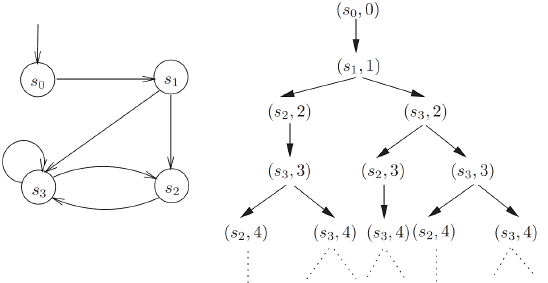
\includegraphics[width=0.9\textwidth]{imagens/ctl_ex.png}
	\caption{Exemplo de árvore de computação num sistema de transição~\cite{huth2004logic}.
		\label{fig:ctl_ex}}
\end{figure}
\FloatBarrier

A sintaxe de construção de fórmulas CTL estende a LTL e adiciona os operadores existencial ($E$) e universal ($A$) consiste em:
\begin{equation}
\begin{align*}
& \varphi ::= \top \mid \perp \mid p \mid \neg \varphi \mid \varphi \wedge \varphi \mid \varphi\vee\varphi \mid \varphi \to \varphi \mid \\ 
& AX\varphi \mid EX\varphi \mid AF\varphi \mid EF\varphi \mid AG\varphi \mid EG\varphi \mid A[\varphi U \varphi]\mid E[\varphi U \varphi]
\end{align*}
\end{equation} 

Os conectivos temporais da CTL são usados em pares. O primeiro conectivo da fórmula é um quantificador, denotado por $A$ (inevitavelmente) ou $E$ (provavelmente), enquanto que o segundo é usado da mesma forma que na LTL. Os operadores temporais $E$ e $A$ expressam propriedades para algum ou todos os caminhos de computação que se iniciam em
determinado estado~\cite{katoen1999concepts}. Alguns exemplos de fórmulas CTL são apresentados a seguir: 
\begin{itemize}
	\item é possível chegar a um estado em que o sistema está $iniciado$ mas não $pronto$? 
	\begin{equation}
	EF(iniciado \wedge \neg pronto)
	\end{equation}
	\item em qualquer caminho e em todo este caminho, se algum recurso é $requisitado$, ele eventualmente é $reconhecido$? 
	\begin{equation}
	AG(requisitado \to AF\;reconhecido)
	\end{equation}
	\item um determinado processo está $habilitado$ infinitamente em cada caminho de computação. 
	\begin{equation}
	AG(AF\;habilitado)
	\end{equation}
\end{itemize}

Assim como na LTL, as fórmulas em CTL são interpretadas sobre os caminhos a partir de estados e um sistema de transição.~\cite{katoen1999concepts}. Cada \textit{path} é entendido como um caminho de estados possível no modelo, em que a raiz da árvore representa o estado inicial. Dado o modelo de transição $\mathcal{M} = (S, \rightarrow, L)$, a relação de satisfação $\mathcal{M}, s \models \equiv$ pode ser dada indutivamente conforme é exibido na Figura~\ref{fig:ctl_sem}, em que $s \in \mathcal{M}$ e $\varphi$ é uma fórmula em CTL~\cite{mura2016}.

\begin{figure}[ht]
	\centering
	\begin{align}
	&\mathcal{M},s  \models  \top \\
	&\mathcal{M},s  \not\models  \perp \\
	&\mathcal{M},s  \models  p \iff p \in L(s) \\
	&\mathcal{M},s  \models  \neg \varphi \iff \pi \not \models \varphi \\
	&\mathcal{M},s  \models  \varphi \wedge \varphi' \iff \mathcal{M},s \models \varphi \mbox{ e } \mathcal{M},s \models \varphi' \\
	&\mathcal{M},s  \models  \varphi \vee \varphi' \iff \mathcal{M},s \models \varphi \mbox{ ou } \mathcal{M},s \models \varphi' \\
	&\mathcal{M},s  \models  \varphi \to \varphi' \iff \mathcal{M},s \not\models \varphi \mbox{ ou } \mathcal{M},s \models \varphi' \\
	&\mathcal{M},s  \models  AX\varphi \iff \forall s_1 \mid s\to s_1 \mbox{ com } \mathcal{M}, s_1 \models \varphi \\
	&\mathcal{M},s  \models  EX\varphi \iff \exists s_1 \mid s\to s_1 \mbox{ com } \mathcal{M}, s_1 \models \varphi \\
	&\mathcal{M},s  \models  AG\varphi \iff \forall \pi = s_1\to s_2\to s_3\to \dots \mid s_1 = s \mbox{ e } \forall s_i \in \pi \mbox{ com } \mathcal{M}, s_i \models \varphi \\
	&\mathcal{M},s  \models  EG\varphi \iff \exists \pi = s_1\to s_2\to s_3\to \dots \mid s_1 = s \mbox{ e } \forall s_i \in \pi \mbox{ com } \mathcal{M}, s_i \models \varphi \\
	&\mathcal{M},s  \models  AF\varphi \iff \forall \pi = s_1\to s_2\to s_3\to \dots \mid s_1 = s \mbox{ e } \exists s_i \in \pi \mid \mathcal{M}, s_i \models \varphi \\
	&\mathcal{M},s  \models  EF\varphi \iff \exists \pi = s_1\to s_2\to s_3\to \dots \mid s_1 = s \mbox{ e } \exists s_i \in \pi \mid \mathcal{M}, s_i \models \varphi \\
	&\mathcal{M},s  \models  A[\varphi U \varphi'] \iff \forall \pi = s_1\to s_2\to s_3\to \dots \mid s_1 = s \exists s_i \in \pi \mid \\
	&\mathcal{M}, s_i \models \varphi' \mbox{ e } \forall j < i \mbox{ com }  \mathcal{M}, s_j \models \varphi \\
	&\mathcal{M},s  \models  E[\varphi U \varphi'] \iff \exists \pi = s_1\to s_2\to s_3\to \dots \mid s_1 = s \exists s_i \in \pi \mid \\
	&\mathcal{M}, s_i \models \varphi' \mbox{ e } \forall j < i \mbox{ com }  \mathcal{M}, s_j \models \varphi
	\end{align}
	\caption{Semântica da CTL.
		\label{fig:ctl_sem}}
\end{figure}
\FloatBarrier

Na CTL, os quantificadores existencial e universal pode ser aninhados para expressar propriedades mais complexas. Por exemplo, uma propriedade em que para todo caminho de computação sempre é possível retornar para o estado inicial, pode ser representada por $AG~(EF~(inicio))$. Assim, interpreta-se que em todo estado do sistema ($G$), para todo caminho de computação ($A$), existe a possibilidade ($E$) de eventualmente retornar ao início ($F~inicio$)~\cite{baier2008principles}.

Outro expressão que não pode ser descrita em LTL é apresentada como segue:
\begin{itemize}
	\item Um elevador pode permanecer parado no 3º andar com as portas fechadas?
\end{itemize}
\begin{align}
& AG(andar3\wedge parado \wedge portaFechada \rightarrow EG(andar3 \wedge parado \wedge portaFechada))
\end{align} 

\section{Cálculo de Processos}

O cálculo de processos envolve um conjunto de abordagens para modelagem formal de sistemas concorrentes que utilizam fórmulas algébricas. Por meio de métodos descritivos de alto nível, possibilita a representação de interações, comunicações e sincronizações entre uma coleção de agentes ou processos independentes. Desta forma, descrições de processos podem ser manipuladas e analisadas, permitindo a formalização do raciocínio sobre equivalências entre processos~\cite{baeten2005brief}.

Mediante ao uso de operadores, são definidas leis algébricas que representam interações entre processos independentes, de forma que as expressões possam ser manipuladas usando raciocínio equacional~\cite{baeten2005brief}.

A seguir são descritos alguns cálculos utilizados para modelagem de processos concorrentes. O Cálculo de Sistemas de Comunicação (CCS)~\cite{milner1986ccs} serve como base para o desenvolvimento do Cálculo-$\pi$~\cite{milner1992calculus, milner1992calculus2}, que por sua vez, possui uma extensão com aspecto temporal denominada TPi~\cite{berger2003two}.

\subsection{Cálculo de Sistemas de Comunicação}

O CCS é um cálculo de processos desenvolvido por~\citeauthor{milner1986ccs} para modelagem de sistemas concorrentes sob duas ideias centrais: comunicação e sincronização~\cite{milner1986ccs}. Para isso, o formalismo utiliza de dois componentes básicos:

\begin{itemize}
	\item \textbf{Agente}: Também chamado de processo, é qualquer sistema concorrente o qual seu comportamento é uma ação discreta;
	\item \textbf{Ação}: É a interação (comunicação) entre dois agentes ou uma interação independente consigo mesmo. Para que a comunicação ocorra, os agentes devem estar sincronizados. 
\end{itemize}

Com um alto nível de articulação e flexibilidade na manipulação, o CCS é aplicável não somente aos processos de \textit{softwares}, mas também à estruturas de dados, e, sob um certo nível de abstração, para sistemas de \textit{hardware}~\cite{milner1986ccs}. 

O cálculo permite que os processos modelados sejam observáveis em função de sua estrutura e funcionamento. Ou seja, seu comportamento pode ser observado enquanto é executado.

Algumas definições são essenciais para a compreensão da estrutura do CCS, são elas:

\begin{itemize}
	\item $\mathcal{K}$ é o conjunto dos nomes dos  processos (constantes);
	\item $\mathcal{A}$ define o conjunto dos canais;
	\item $\mathcal{L} = \mathcal{A} \cup \mathcal{\overline{A}}$ representa o conjunto dos rótulos, onde $\mathcal{\overline{A}} = \overline{a} | a \in \mathcal{A}$. Elementos de $\mathcal{A}$ são chamados de canais e os de $\mathcal{\overline{A}}$ são os co-canais;
	\item $Act = \mathcal{L} \cup \{\tau\}$ denota o conjunto das ações, onde $\tau$ representa uma ação nula;
	\item O conjunto dos termos que definem um processo (expressão do processo), é denotado por $\mathcal{P}$. 		
\end{itemize}

Com isso, a sintaxe da CCS é apresentada conforme segue:

\begin{equation}
	P := K~|
	~\alpha.P~|
	~\Sigma_{i\in I}~P_{i}~|
	~P_{1} | P_{2}~|
	~P \setminus L~|
	~P[f]~|
	~\textit{\underline{if}}~\textit{true}~\textit{\underline{then}}~P~\textit{\underline{else}~F}
\end{equation}

O CCS é baseado nos elementos: constante de processo $K \in \mathcal{K}$; ação prefixada $\alpha.P$ (lê-se: $\alpha$, então $P$), onde $\alpha \in Act$ e $P \in \mathcal{P}$; somatório $\Sigma_{i\in I} P_{i}~|~P_{1}$, no qual $P_{1} + P_{2} = \Sigma_{i\in \{1,2\}}~P_{i}$, que representa uma escolha não determinística entre $P_{1}$ ou $P_{2}$ ($P_{1}, P_{2} \in \mathcal{P}$); composição paralela $P_{1} | P_{2}$, representa que os processos $P_{1}$ e $P_{2}$ estão executando paralelamente e encontram-se prontos para se comunicar; restrição $P \setminus L$ (lê-se: $P$ restringido por $L$), sendo que $L \subseteq \mathcal{A}$; renomeação $P[f]$ (lê-se: $P$ renomeado por f), dado que $P \in \mathcal{P}$ e $f$ é uma função de renomeação denotada por $f : Act \longrightarrow Act$, em que $f(\tau) = \tau$ e $f(\overline{a}) = \overline{f(a)}$; condição $\textit{\underline{if}}~\textit{true}~\textit{\underline{then}}~P~\textit{\underline{else}}~F$, no qual \textit{true} indica que uma dada condição que pode ser verdadeira ou não.    

A fim de evitar o uso excessivo de parênteses e organizar a interpretação sobre as expressões dos processos, é dada a seguinte regra de procedência de operadores:

\begin{align*}
 &\{Restrição, Renomeação\} > Ação > Composição > Somatório
\end{align*}

Portanto, por exemplo:
\begin{equation}
P~|~\tau.Q\setminus\alpha~+~R[f]~=~(P~|~(\tau.(Q\setminus\alpha)))~+~(R[f]) 
\end{equation}

Um sistema em CCS consiste num conjunto de definições de equações na forma $K~\stackrel{def}{=}P~$, sendo que $K \in \mathcal{K}$ é uma constante de processo e $P \in \mathcal{P}$ é a expressão que define um processo. O formalismo permite que cada constante de processo tenha apenas uma expressão, no qual a recursão é permitida, por exemplo: $P~\stackrel{def}{=}~\overline{a}.P~|A~$.

A semântica do CCS é determinada por um Sistema de Transições Rotuladas (LTS) composto relações binárias do tipo $\stackrel{\alpha}{\longrightarrow}$, em que $\alpha \in Act\cup\{\tau\}$.

A partir de uma coleção de equações de definição, tem-se um LTS na forma ($Proc, Act, \{\stackrel{a}{\longrightarrow}|~a \in Act\}$), no qual seus elementos são descritos respectivamente como:

\begin{itemize}
	\item $Proc = \mathcal{P}$: conjunto de todas as expressões de processo;
	\item $Act = \mathcal{L}\cup\{\tau\}$: conjunto de todas as ações, inclusive a ação nula $\tau$;
	\item $\{\stackrel{a}{\longrightarrow}|~a \in Act\}$: Relação de transição dada por regras de uma Semântica Operacional Estrutural na forma:
\begin{equation}
regra~\dfrac{premissa}{conclusão}~condições 
\end{equation}	
\end{itemize}

As transições denotadas na Tabela~\ref{tab:pi_sos} podem gerar derivações capazes de serem computadas por meio de uma árvore de derivação, como ilustrado na Figura~\ref{fig:ccs_tree}, considerando os seguintes processos e suas definições:

\begin{align}
&A \stackrel{def}{=} a.A', \nonumber \\
&A' \stackrel{def}{=} \overline{c}.A, \nonumber \\
&B \stackrel{def}{=} c.B', \nonumber \\
&B' \stackrel{def}{=} \overline{b},B
\end{align}

\begin{figure}[ht]
	\centering
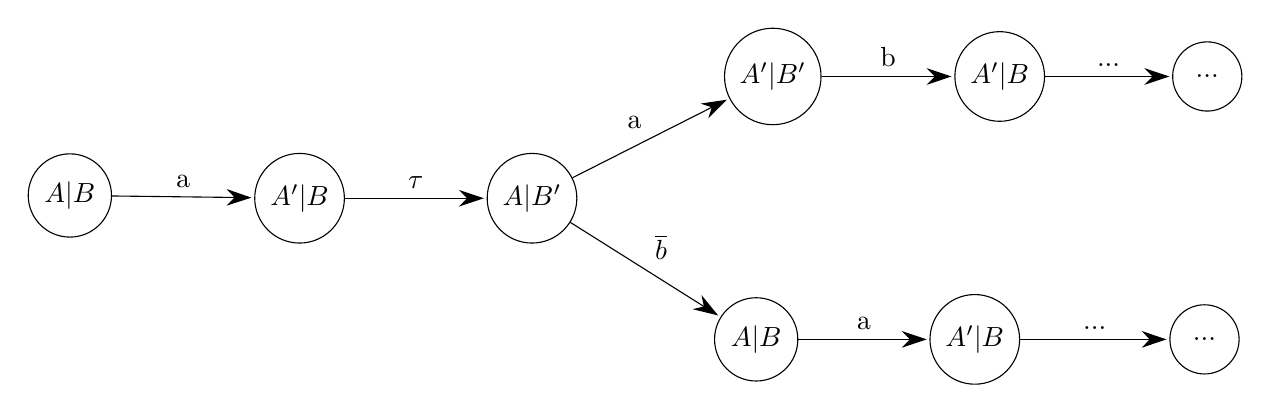
\begin{tikzpicture}[>={Stealth[width=6pt,length=9pt]}, accepting/.style={double distance = 2pt, outer sep = 1pt + \pgflinewidth}, shorten >=1pt, auto]
\draw (109.0pt, -125.0pt)node[state](0){$A|B$};
\draw (192.0pt, -126.0pt)node[state](1){$A'|B$};
\draw (276.0pt, -126.0pt)node[state](2){$A|B'$};
\draw (363.0pt, -82.0pt)node[state](3){$A'|B'$};
\draw (357.0pt, -177.0pt)node[state](4){$A|B$};
\draw (445.0pt, -82.0pt)node[state](5){$A'|B$};
\draw (436.0pt, -177.0pt)node[state](6){$A'|B$};
\draw (520.0pt, -82.0pt)node[state](7){$...$};
\draw (519.0pt, -177.0pt)node[state](8){$...$};
\path[->] (3) edge node{b}(5);
\path[->] (5) edge node{...}(7);
\path[->] (2) edge node{a}(3);
\path[->] (0) edge node{a}(1);
\path[->] (4) edge node{a}(6);
\path[->] (1) edge node{$\tau$}(2);
\path[->] (2) edge node{$\overline{b}$}(4);
\path[->] (6) edge node{...}(8);
\end{tikzpicture}	
	\caption{Exemplo de árvore de computação num sistema de transição.
		\label{fig:ccs_tree}}
\end{figure}
\FloatBarrier

\begin{table}[!ht]
	\centering\tiny{
		\caption{Semântica Estrutural Operacional do CCS~\cite{milner1986ccs}.} \label{tab:ccs_sos}}
\begin{tabular}{|c|c|c|}
	\hline 
	\textbf{Regra} & $\dfrac{\textbf{premissa}}{\textbf{conclusão}}$ & \textbf{Condição} \\ 
	\hline 
	Prefixo & $\dfrac{}{\alpha.P\stackrel{\alpha}{\longrightarrow}P}$ & - \\ 
	\hline 
	Somatório$_{j}$ & $\dfrac{P_{j}\stackrel{\alpha}{\longrightarrow}P'_{j}}{\Sigma_{i\in I}~P_{i}\stackrel{\alpha}{\longrightarrow}P'_{j}}$ & $j \in I$ \\ 
	\hline 
	Composição 1 & $\dfrac{P \stackrel{\alpha}{\longrightarrow}P'}{P|Q\stackrel{\alpha}{\longrightarrow}P'|Q}$ & - \\ 
	\hline 
	Composição 2 & $\dfrac{Q\stackrel{\alpha}{\longrightarrow}Q'}{P|Q\stackrel{\alpha}{\longrightarrow}P|Q'}$ & - \\ 
	\hline 
	Composição 3 & $\dfrac{P\stackrel{a}{\longrightarrow}P'~~Q\stackrel{\overline{a}}{\longrightarrow}Q'}{P|Q\stackrel{\tau}{\longrightarrow}P'|Q'}$ & - \\ 
	\hline 
	Restrição & $\dfrac{P\stackrel{\alpha}{\longrightarrow}P'}{P\setminus L\stackrel{\alpha}{\longrightarrow}P'\setminus L}$ & $\alpha, \overline{\alpha} \notin L$ \\ 
	\hline 
	Renomeação & $\dfrac{P\stackrel{\alpha}{\longrightarrow}P'}{P[f]\stackrel{f(\alpha)}{\longrightarrow}P'[f]}$ & - \\ 
	\hline 
	Condicional $if_{1}$ & $\dfrac{P\stackrel{\alpha}{\longrightarrow}P'}{\textit{\underline{if}}~\textit{true}~\textit{\underline{then}}~P~\textit{\underline{else}}~Q\stackrel{\alpha}{\longrightarrow}P'}$ & $if~true$ \\ 
	\hline 
	Condicional $if_{2}$ & $\dfrac{Q\stackrel{\alpha}{\longrightarrow}Q'}{\textit{\underline{if}}~\textit{true}~\textit{\underline{then}}~P~\textit{\underline{else}}~Q\stackrel{\alpha}{\longrightarrow}Q'}$ & $if\neg true$ \\ 
	\hline 
	Definição & $\dfrac{(P\{y_{i}/x_{i}\})\stackrel{\alpha}{\longrightarrow}P'}{K(y_{i})\stackrel{f(\alpha)}{\longrightarrow}P'}$ & $fornece~K(x_{i})\stackrel{def}{=} P$ \\ 
	\hline 
\end{tabular} 
\end{table} 

Uma característica presente no CCS é a passagem de valores, que permite que valores específicos possam ser enviados ou recebidos pelos processos (e.g., inteiros e \textit{Strings}). Para isso, ações que representam canais e co-canais são utilizadas na notação prefixada com a forma $a(x).P$ ou $\overline{a}(x).P$, a qual $x$ simboliza um valor arbitrário a ser transmitido ou rebebido. Os canais $\mathcal{A}$ e os co-canais $\mathcal{\overline{A}} = \{\overline{a}|a \in \mathcal{A}\}$ caracterizam os canais de recepção e saída dos valores, respectivamente.

Na Figura~\ref{fig:ccs_value} são apresentados exemplos de passagem de valor, em que é aplicada uma troca de valor simples e outra infinita, de acordo com os processos modelados abaixo.

\begin{align}
&P \stackrel{def}{=} in(x).P'(x) \nonumber \\
&P'(x) \stackrel{def}{=} \overline{out}(x).P
\end{align}
\begin{align}
&P \stackrel{def}{=} \sum_{i \in \mathbb{N}} in(i).C'_{i} \nonumber \\
&C'_{i} \stackrel{def}{=} \overline{out}(i).C
\end{align}

\begin{figure}[ht]
	\centering
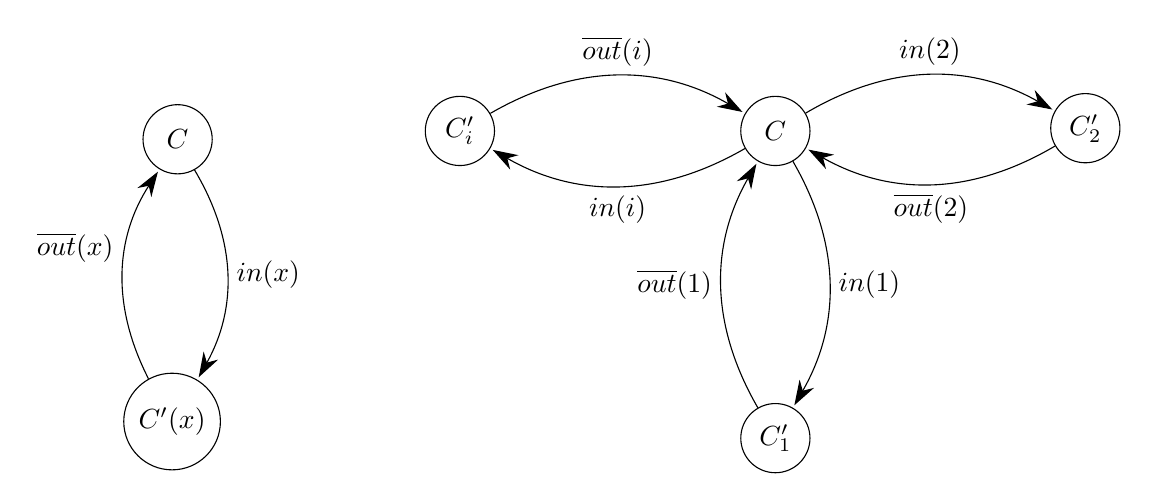
\begin{tikzpicture}[>={Stealth[width=6pt,length=9pt]}, accepting/.style={double distance = 2pt, outer sep = 1pt + \pgflinewidth}, shorten >=1pt, auto]
\draw (75.0pt, -49.0pt)node[state](0){$C$};
\draw (73.0pt, -151.0pt)node[state](1){$C'(x)$};
\draw (177.0pt, -46.0pt)node[state](2){$C'_{i}$};
\draw (291.0pt, -46.0pt)node[state](3){$C$};
\draw (403.0pt, -45.0pt)node[state](4){$C'_{2}$};
\draw (291.0pt, -157.0pt)node[state](5){$C'_{1}$};
\path[->] (2) edge[bend left] node{$\overline{out}(i)$}(3);
\path[->] (5) edge[bend left] node{$\overline{out}(1)$}(3);
\path[->] (4) edge[bend left] node{$\overline{out}(2)$}(3);
\path[->] (0) edge[bend left] node{$in(x)$}(1);
\path[->] (3) edge[bend left] node{$in(i)$}(2);
\path[->] (3) edge[bend left] node{$in(2)$}(4);
\path[->] (1) edge[bend left] node{$\overline{out}(x)$}(0);
\path[->] (3) edge[bend left] node{$in(1)$}(5);
\end{tikzpicture}
	\caption{Passagem de valores em CSS.
		\label{fig:ccs_value}}
\end{figure}
\FloatBarrier 

\subsection{Cálculo-$\pi$}

O Cálculo-$\pi$, desenvolvido por~\citeauthor{milner1992calculus}, é uma extensão do CCS, no qual aspectos de mobilidade são acrescentados e sua complexidade é reduzida, reforçando sua teoria básica, enquanto preserva suas propriedades algébricas~\cite{milner1992calculus}.

Com este formalismo, os nomes dos canais (ou \textit{links}) aparecem como parâmetros na comunicação, portanto, vai além do CCS. Apesar da adição de variáveis aos canais, bem como sobre valores de dados comuns, o cálculo não tornou-se mais complexo. De fato, todas as distinções entre nomes de canais, variáveis e demais dados foram removidas, e, portanto, todos são chamados de $names$. Logo, tem-se duas classes de entidades: $names$ e agentes~\cite{milner1992calculus}.

Para quaisquer definições adiante, pressupõe-se que $x$, $y$, $z$, $w$, $v$ e $u$ são metavariáveis representadas por nomes, pertencentes ao conjunto $\mathcal{N}$ de nomes. Presume-se também que há um conjunto de identificadores de agente, em que cada identificador $A$ possui aridade maior ou igual a zero. $P$, $Q$ e $R$ representam o conjunto do comportamento de um agente.

A sintaxe dos agentes pode ser resumida como segue:

\begin{equation}
P ::=~0~
|~\overline{y}x.P~
|~y(x).P~
|~\tau.P~
|~(x)P~
|~[x = y]P~
|~P_{1}|P_{2}~
|~P_{1} + P_{2}~
|~A(y_{1}, ..., y_{n})
\end{equation}

Considera-se que $0$ é um operador nulo. Os operadores $\overline{x}y.$, $x(y).$, $\tau.$, $(x)$, e $[x=y]$ são unários, enquanto que $|$ e $+$ são binários, e $n$ indica a aridade de $A$~\cite{milner1992calculus2}. 

Para cada agente nas formas $\overline{y}x.P$ e $y(x).P$, a ocorrência de $y$ entre parênteses é chamada de ocorrência de ligação. Uma ocorrência de $y$ de um agente é considerada "livre" se a mesma não estiver no âmbito de uma ocorrência de ligação. Portanto, o conjunto de nomes livres (\textit{free names}) em $P$ é denotado por $fn(P)$.

O operador de correspondência $[x = y]P$ indica que o agente irá se comportar como $P$ caso os nomes $x$ e $y$ sejam idênticos. Caso contrário, agirá como $0$.

Uma equação de definição de um identificador de agente $A$ é dada por $$A(x_{1}, ..., x_{n})\stackrel{def}{=}P,$$

em que os elementos do tipo $x_{i}$ são distintos e $fn(P)\subseteq \{x_{1}, ..., x_{n}\}$.

Se uma ocorrência de um nome em um agente não é livre, então é chamado de nome "vinculado" (\textit{bound names}). Assume-se $bn(P)$ como o conjunto de nomes vinculados de $P$. Se $A (\tilde{x})\stackrel{def}{=} Q$, então $bn(A (\tilde{x})) = bn(Q)$, no qual $\tilde{x} = x_{1}, ..., x_{n}$. Portanto, $n(P)$ representa o conjunto $fn(P) \cup bn(P)$ dos nomes contidos em $P$.

A substituição é uma função $\sigma$ de $\mathcal{N}$ pra $\mathcal{N}$ em que, quando $x_{i}\sigma = y_{i}$, no qual $1\leq i \leq n$ (e $x\sigma = x$ para os demais nomes $x$), pode-se escrever $\{y_{1}/x_{1}, ..., y_{n}/x_{n}\}$ ou $\{\tilde{y}/\tilde{x}\}$ para $\sigma$. Ou seja, para todo $x_{i}$ haverá um $y_{i}$ que substituirá seu valor.

As ações do Cálculo-$\pi$ podem ser observadas por meio de um LTS, assim como no CCS. este formalismo define 4 quatro tipos de ações $\alpha$:
\begin{itemize}
	\item \textbf{Ação nula $\tau$}: $P \stackrel{\tau}{\longrightarrow} Q$ expressa que $P$ pode envolver $Q$ de forma que isso exija alguma interação com o ambiente. As ações nulas podem surgir na forma $\tau.P$, e também em comunicações entre agentes;
	\item \textbf{Saída livre $\overline{a}y$}: $P \stackrel{\overline{a}y}{\longrightarrow} Q$ implica que $P$ emite o nome livre $y$ pela porta de saída $\overline{x}$ e é representada pela forma prefixada $\overline{x}y.P$;
	\item \textbf{Entrada $x(y)$}: $P \stackrel{x(y)}{\longrightarrow} Q$ define que $P$ recebe qualquer nome $w$ pela porta $x$, que envolve $Q\{w/y\}$. Enquanto que em CCS, a ação de entrada contêm o valor atual a ser recebido, no Cálculo-$\pi$ $y$ representa uma referência ao local onde nome recebido deve ir. Tal ação pode mostrar-se na forma $x(y).P$;
	\item \textbf{Saída vinculada $\overline{x}(y)$}: $P \stackrel{\overline{x}(y)}{\longrightarrow} Q$ denota que $P$ emite um nome particular (i.e., um nome vinculado de $P$) pela porta de saída $\overline{x}$, em que $(y)$ é a referência de onde o nome particular ocorre. Ações de saída vinculadas está presente em ações de saída livre que carregam nomes fora de seu escopo, por exemplo, em $(y)\overline{x}y.P$.
\end{itemize}

A semântica do Cálculo-$\pi$ é apresentada na Figura~\ref{fig:pi_semant}, e, assim como no CCS, é declarada por meio de uma Semântica Operacional Estrutural que leva em conta as relações de transição de seus operadores.

\begin{table}[!ht]
	\centering\tiny{
		\caption{Semântica Operacional Estrutural do Cálculo-$\pi$~\cite{milner1992calculus2}. \label{tab:pi_sos}}
\begin{tabular}{|c|c|c|}
	\hline 
	\textbf{Regra} & $\dfrac{\textbf{premissa}}{\textbf{conclusão}}$ & \textbf{Condição} \\ 
	\hline 
	Ação vazia & $\dfrac{\_}{\tau.P\stackrel{\tau}{\longrightarrow}P}$ & - \\ 
	\hline 
	Ação de saída livre & $\dfrac{\_}{\overline{x}y.P\stackrel{\overline{x}y}{\longrightarrow}P}$ & - \\ 
	\hline 
	Ação de entrada & $\dfrac{\_}{x(z).P\stackrel{x(w)}{\longrightarrow}P\{w/z\}}~w \notin fn((z)P)$ & - \\ 
	\hline 
	Somatório & $\dfrac{P\stackrel{\alpha}{\longrightarrow}P'}{P + Q\stackrel{\alpha}{\longrightarrow}P'}$ & - \\ 
	\hline 
	Correspondência & $\dfrac{P\stackrel{\alpha}{\longrightarrow}P'}{[x = x] P \stackrel{\alpha}{\longrightarrow}P'}$ & - \\ 
	\hline 
	Identificador & $\dfrac{P\{\tilde{y}/\tilde{x}\}\stackrel{\alpha}{\longrightarrow}P'}{A(\tilde{y})\stackrel{\alpha}{\longrightarrow}P'}$ & $A(\tilde{x})\stackrel{def}{=}P$ \\ 
	\hline 
	Composição paralela & $\dfrac{P\stackrel{\alpha}{\longrightarrow}P'}{P|Q\stackrel{\alpha}{\longrightarrow}P'|Q}$ & $bn(\alpha)\cap fn(Q) = \varnothing$ \\ 
	\hline 
	Comunicação & $\dfrac{P\stackrel{\overline{x}y}{\longrightarrow}P'~~Q\stackrel{x(z)}{\longrightarrow}Q'}{P|Q\stackrel{\tau}{\longrightarrow}P'|Q'\{y/z\}}$ & - \\ 
	\hline 
	Fechamento de escopo & $\dfrac{P\stackrel{\overline{x}(w)}{\longrightarrow}P'~~Q\stackrel{x(w)}{\longrightarrow}Q'}{P|Q\stackrel{\tau}{\longrightarrow}(w)(P'|Q')}$ & - \\ 
	\hline 
	Abertura de escopo & $\dfrac{P \stackrel{\overline{x}y}{\longrightarrow}}{(y)P\stackrel{\overline{x}(w)}{\longrightarrow}P'\{w/y\}}$ & $y\neq x, w \notin fn((y)P')$ \\ 
	\hline 
	Restrição & $\dfrac{P\stackrel{\alpha}{\longrightarrow}P'}{(y)P\stackrel{\alpha}{\longrightarrow}(y)P'}$ & $y \notin n(\alpha)$ \\ 
	\hline 
\end{tabular} 
	}
\end{table}

Um sistema em Cálculo-$\pi$ pode ser representado por meio de um grafo de fluxo. Supõe-se que um agente $P$ deseja transferir para um novo agente $Q$ a tarefa de transmitir o valor 5 para $R$. Para isso, presume-se que $P$ está conectado ao $Q$, inicialmente, por meio de um canal $b$.

Portanto, tem-se $P \equiv \overline{b}a.\overline{b}5.P'$, no qual tanto o canal $a$ quanto o valor 5 são transmitidos ao longo de $a$. Sendo assim, o processo $Q \equiv b(y).b(z).\overline{y}z.\textbf{0}$, o qual recebe, em ordem, um canal e um valor através de $b$, e então transmite o valor pelo canal, e, por fim, é encerrado. O sistema completo é expressado a seguir:
\begin{equation} \label{eq:pi_ex}
 (\overline{b}a.\overline{b}5.P'~|~b(y).b(z).\overline{y}z.\textbf{0}~|~a(x).R')\setminus a \setminus b ~ \stackrel{\tau}{\longrightarrow} ~ (P'~|~\overline{a}5.\textbf{0}~|~a(x).R')\setminus a \setminus b
\end{equation}

A Figura~\ref{fig:pi_graph} a seguir apresenta o grafo de fluxo do sistema:

\begin{figure}[ht]
	\centering
	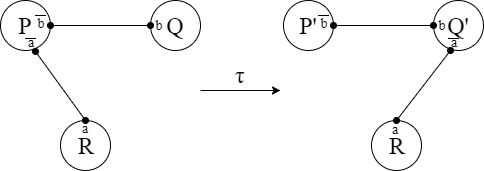
\includegraphics[width=0.8\textwidth]{imagens/calc_pi_ex.png}
	\caption{Grafo de fluxo do sistema (\ref{eq:pi_ex})~\cite{milner1992calculus}.
		\label{fig:pi_graph}}
\end{figure}
\FloatBarrier

\subsection{Álgebra temporal de processos TPi} \label{sec:tpi}
    
A TPi é uma álgebra temporal de processos inspirada no Cálculo-$\pi$~\cite{milner1992calculus, milner1992calculus2} e desenvolvida por~\citeauthor{berger2003two}. O formalismo apresenta um cálculo para transmissão síncrona de mensagens capaz de expressar entradas cronometradas~\cite{aziz2016formal}.

A sintaxe da linguagem define processos $P, Q \in \mathcal{P}$, baseado nos nomes $x, y \in \mathcal{N}$ como segue:

\begin{equation}
P, Q ::= \overline{x}\langle y \rangle.P~|~
timer^{t}(x(y).P,Q)~|~
!P~|~
(vx)P~|~
(P|Q)~|~
(P+Q)~|~
\textbf{0}~|~
A(x)
\end{equation}

A sintaxe corresponde aos operadores do Cálculo-$\pi$, exceto pelas ações de entrada representadas com o acréscimo de um cronômetro, de forma $timer^{t}(x(y).P,Q)$, em que $t \in \mathbb{N}$ simboliza um tempo limite, o qual é decrementado de acordo com o ambiente do processo, podendo $t$ assumir qualquer unidade de tempo. Desta forma, enquanto $t > 0$, a ação de entrada $x(y).P$ pode atuar paralelamente com ações de saída. Em contrapartida, quando $t = 0$, o processo age como $Q$~\cite{aziz2016formal}.

Chamadas de definição de processos são expressas na forma $A(x)$, as quais invocam uma definição de processo $A(y)\stackrel{def}{=}P$, enquanto que o valor $x$ é passado e substitui $y$. Como a definição $A$ não aceita quaisquer parâmetros de entrada, o parâmetro $y$ é omitido. Assim, a definição é escrita como $A()\stackrel{def}{=}P$~\cite{aziz2016formal}.

A Semântica Operacional Estrutural da TPi é dada em termos de sua congruência estrutural $\equiv$, e a relação de suas transições rotuladas $\stackrel{\alpha}{\longrightarrow}$ é apresentada na Tabela~\ref{tab:tpi_sos}, em que $fn(P)$ denota o conjunto de nomes livres de $P$.

Definições de $\equiv$ são padronizadas~\cite{milner1992calculus2}, exceto pelas regras~\ref{eq:6},~\ref{eq:7},~\ref{eq:8} e~\ref{eq:9}, as quais lidam com cronômetros zerados e infinitos, e chamadas de definição de processos parametrização e não parametrizadas, respectivamente.

Os rótulos $\alpha \in \{\stackrel{\overline{x}\langle y \rangle}{\longrightarrow}, \stackrel{\overline{x}(y)}{\longrightarrow}, \stackrel{x(z)}{\longrightarrow}, \stackrel{\tau}{\longrightarrow}\}$, expressam saídas livres e vinculadas, entradas e ações nulas. 

As regras de transição $\stackrel{\alpha}{\longrightarrow}$ são descritas detalhadamente por~\cite{berger2003two}, exceto pela regra~\ref{eq:19}, que define uma função de passagem de tempo $\eth : \mathcal{P} \longrightarrow \mathcal{P}$, que expressa a marcação de tempo dos cronômetros ativos, no qual uma entrada temporizada está aguardando a aceitação de uma mensagem, em que:

$\eth(P)=$
\begin{cases}
	\text{$timer^{t}(x(y).Q,Q')$}, & \text{$se~P = timer^{t+1}(x(y).Q,Q')$}, \\
	& \text{$e~0<t+1<\infty$} \\
	\text{$\eth(Q)|\eth(R)$}, & \text{$se~P=Q|R$} \\
	\text{$\eth(Q) + \eth(R)$}, & \text{$se~P = Q + R$} \\
	\text{$(vx)\eth(Q)$}, & \text{$se~P = (vx)Q$} \\
	\text{$\eth(Q[x/y])$}, & \text{$se~P = A(x)~e~A(y) \stackrel{def}{=} Q$} \\
	\text{$\eth(Q)$}, & \text{$se~P = A()~e~A() \stackrel{def}{=} Q$} \\
	\text{$P$}, & \text{outra forma}
\end{cases} 

\begin{figure}[ht]
	\centering
	\begin{align}
		&\textbf{Regras~da~relação}~\equiv: \nonumber \\
		& \mathcal{P}/ \equiv, |, \textbf{0})~é~um~monóide~comutativo \\
		& (vx)\textbf{0} \equiv \textbf{0} \\
		& (vx)(vy)P \equiv (vy)(vx)P \\
		& !P \equiv P|!P \\
		& (vx)(P|Q) \equiv (P|(vx)Q) se x \notin fn(Q) \\ 
		& timer^{0}(x(z).P,Q) \equiv Q \label{eq:6} \\ 
		& timer^{\infty}(x(z).P,Q) \equiv x(z).P \label{eq:7} \\
		& A(x) \equiv P[x/y],~em~que~A(y) \stackrel{def}{=} P \label{eq:8} \\
		& A() \equiv P,~em~que~A() \stackrel{def}{=} P \label{eq:9} \\
		& \nonumber \\
		&\textbf{Regras~da~relação}~\stackrel{\alpha}{\longrightarrow}: \nonumber \\
		& \overline{x}\langle y \rangle.P \stackrel{\overline{x}\langle y \rangle}{\longrightarrow} P \\		
		& timer^{t+1}(x(z).P,Q) \stackrel{x(z)}{\longrightarrow} P \\
		& P \stackrel{\overline{x}\langle y \rangle}{\longrightarrow} Q ~~ \Rightarrow ~~ (vy)P \stackrel{\overline{x}(y)}{\longrightarrow} se~ x \neq y \\
		& P \stackrel{\overline{x}\langle y \rangle}{\longrightarrow} P', Q \stackrel{x(z)}{\longrightarrow} Q' ~~ \Rightarrow ~~ P|Q \stackrel{\tau}{\longrightarrow} P' | Q'[y/z] \\
		& P \stackrel{\overline{x}(y)}{\longrightarrow} P', Q \stackrel{x(z)}{\longrightarrow} Q' ~~ \Rightarrow ~~ P|Q \stackrel{\tau}{\longrightarrow} (vy)(P'|Q'[y/z]) \\
		& P \stackrel{\alpha}{\longrightarrow} Q ~~ \Rightarrow ~~ (vx)P \stackrel{\alpha}{\longrightarrow} (vx)Q~se~ x \neq fn(\alpha) \\
		& P \stackrel{\alpha}{\longrightarrow} P' ~~ \Rightarrow ~~ P|Q \stackrel{\alpha}{\longrightarrow} P'|Q \\
		& P \stackrel{\alpha}{\longrightarrow} P' ~~ \Rightarrow ~~ P + Q\stackrel{\alpha}{\longrightarrow} P' \\
		& P \stackrel{\alpha}{\longrightarrow} P' ~~ \Rightarrow ~~ Q + P\stackrel{\alpha}{\longrightarrow} P' \\ \label{eq:19}
		& P \stackrel{\tau}{\longrightarrow} \eth  (P)
	\end{align}
	\caption{Semântica da LTL.
		\label{fig:ltl_sema}}
\end{figure}
\FloatBarrier




\chapter{Trabalhos Relacionados}

Uma abordagem para modelagem do protocolo MQTT escrita em TPi~\cite{berger2003two}, foi proposta por~\citeauthor{aziz2016formal}. Se por um lado, a TPi oferece um alto nível de abstração da comunicação concorrente entre múltiplos agentes, por outro, a mesma não é capaz de formalizar informações importantes como descrição detalhada das ações, conteúdo das mensagens e ordenação da execução dos sistemas.

Um contrato multilateral consiste num conjunto de compromissos envolvendo o acordo entre múltiplos agentes para garantir o cumprimento de cláusulas, a fim de satisfazer as vontades das partes envolvidas, formalizando assim, uma relação contratual. O modelo de contrato multilateral proposto por~\citeauthor{xu2004multi}, oferece um alto nível de detalhamento das relações existentes entre os agentes e suas ações, permitindo a formalização completa do contrato, além de proporcionar a possibilidade da aplicação de um método de monitoramento reativo para detecção das partes responsáveis por violações contratuais~\cite{xu2004multi, xu2005detection}.

A seguir são apresentados os trabalhos que estão mais intimamente relacionados com esta pesquisa. Inicialmente é apresentada a técnica de modelagem do protocolo MQTT e posteriormente técnicas para formalização, monitoramento reativo e detecção de violação de contratos multilaterais.  

\section{Especificação formal de um protocolo de IoT} \label{sec:mqtt_model}

Devido ao crescimento e popularização da IoT, estima-se que bilhões de novos dispositivos estejam interconectados num futuro próximo, gerando bilhões em receita e promovendo maior conforto e bem estar na vida dos usuários, além de otimizar processos industriais e outras aplicações. Tais fatores potencializam a proliferação e demanda por equipamentos com baixo poder de processamento e armazenamento, como sensores e leitores RFID. Com base nisso, são impulsionados os esforços pela padronização da comunicação M2M. Assim, protocolos de comunicação como o MQTT~\cite{mqttv3.1.1}, XMPP~\cite{xmpp2011extensible}, CoAP~\cite{shelby2014constrained} e outros, surgiram como solução para lidar com a comunicação entre dispositivos inseridos no ambiente de IoT~\cite{aziz2016formal}.

Aplicações em IoT podem carecer de um alto nível de confiança em termos de corretude das especificações dos sistemas e assegurar que propriedades não funcionais sejam cumpridas, como segurança e privacidade. Sendo assim, é de suma importância a adoção de métodos formais de análise que garantam que as especificações tenham o mínimo de ambiguidade possível, oferecendo maior confiança e robustez para aplicações que adotam tais especificações~\cite{aziz2016formal}. Diante desta questão, foi proposto por~\citeauthor{aziz2016formal} uma método para modelagem e análise do protocolo MQTT, que auxilia na compreensão do comportamento operacional do protocolo, bem como na detecção de ambiguidades presentes na sua especificação.

\subsection*{Modelagem}

O comportamento operacional do protocolo foi modelado com base nas especificações descritas em sua documentação~\cite{mqttv3.1.1} por meio de um cálculo temporal de processos chamado TPi~\cite{berger2003two}, descrito na Seção~\ref{sec:tpi}. O modelo é baseado na entrega de pacotes PUBLISH, de acordo com os níveis de QoS oferecidos no MQTT, cujas características são discutidas na Seção~\ref{sec:qos}. A modelagem completa é exposta na Figura~\ref{fig:mqtt_model}.

\begin{figure}[ht]
	\centering
\begin{align}
&\textbf{QoS~nível~0:} \nonumber \\
&\quad Cliente(Publish)~|~Servidor(),~em~ que: \nonumber \\
&\quad Cliente(z) \stackrel{def}{=} \overline{c}\langle z \rangle \nonumber \\
&\quad Servidor() \stackrel{def}{=} c(x).\overline{pub}\langle x \rangle \label{eq:qos0} \\
& \nonumber \\
&\textbf{QoS~nível~1:} \nonumber \\
&\quad Cliente(Publish)~|~Servidor(),~em~ que: \nonumber \\
&\quad Cliente(z) \stackrel{def}{=} \overline{c}\langle z \rangle.timer^{t}(c'(y),Cliente(Publish_{DUP}) \nonumber \\
&\quad Servidor() \stackrel{def}{=} !c(x).\overline{pub}\langle x \rangle . \overline{c'} \langle Puback \rangle \\
& \nonumber \\
&\textbf{QoS~nível~2:} \nonumber \\
&\quad Cliente(Publish)~|~Servidor(),~em~ que: \nonumber \\
&\quad Cliente(z) \stackrel{def}{=} \overline{c}\langle z \rangle.timer^{t}(c(y).ClienteCont(y), Cliente(Publish_{DUP})) \nonumber \\
&\quad ClienteCont(u) \stackrel{def}{=} \overline{c'}\langle Pubrel_{u} \rangle . timer^{t'} (c'(w), ClienteCont(u)) \nonumber \\
&\quad Servidor() \stackrel{def}{=} !c(l).(ServidorLate(l) + ServidorEarly(l)) \nonumber \\
&\quad ServidorLate(x) \stackrel{def}{=} (\overline{c}\langle Pubrec_{x} \rangle.c'(v).\overline{pub}\langle x \rangle.\overline{c'}\langle Pubcomp_{v} \rangle.!(c'(v').\overline{c'}\langle Pubcomp_{v'} \rangle)) \nonumber \\
&\quad ServidorEarly(x) \stackrel{def}{=} (\overline{pub}\langle x \rangle.c'(v).\overline{pub}\langle x \rangle.\overline{c}\langle Pubrec_{x} \rangle.c'(q).\overline{c'}\langle Pubcomp_{q} \rangle. \nonumber \\
&\quad \quad \quad \quad \quad \quad \quad \quad \quad \quad \quad \quad \quad \quad \quad \quad \quad \quad \quad \quad \quad \quad \quad \quad  !(c'(q').\overline{c'}\langle Pubcomp_{q'} \rangle))
\end{align}
	\caption{Modelo do protocolo MQTTv3.1.1 em TPi baseado nos três níveis de QoS~\cite{aziz2016formal}, adaptado pelo autor.
		\label{fig:mqtt_model}}
\end{figure}
\FloatBarrier

\section{Um modelo para contratos multilaterais} \label{sec:trab_contratos}

A execução de contratos entre múltiplas partes de negócio representam um ofício relevante dentro da economia global, em que atividades ao longo da cadeia de valor são executadas de forma independente porém cooperativamente entre as companhias~\cite{xu2004monitoring}. Sendo assim, é de suma importância que as partes envolvidas em uma relação contratual cumpram com as cláusulas das quais são responsáveis, e, em caso de não cumprimento, ou seja, quando há uma violação do contrato, o responsável pela violação deve ser identificado.

Uma forma de identificar o responsável por uma violação baseia-se em "quebrar" o contrato num conjunto de contratos bilaterais, e então apontar o responsável, já que essa é uma tarefa relativamente mais simples de ser executada em contratos bilaterais. Porém, pesquisas como a de~\citeauthor{haugen2002multi} demonstram que, apesar da ideia parecer viável, em um relacionamento multilateral complexo, onde há uma série de dependências envolvendo múltiplos agentes, essa conversão pode resultar na perda ou ocultação de informação.

Diante disso, foi proposto por~\citeauthor{xu2004multi} um modelo de contrato multilateral capaz de representar relações contratuais complexas entre múltiplos agentes, assim como realizar o monitoramento do contrato e identificar os responsáveis por violações.

%As definições e conceitos envolvidos são exemplificador por meio de um estudo de caso que envolve a celebração de um contrato multilateral que abrange as partes envolvidas no serviço de uma seguradora de veículos.

\subsection*{Modelo de contrato multilateral}

De acordo com~\citeauthor{xu2004multi}, um contrato é o acordo entre duas ou mais partes baseado em compromissos mútuos. Assim, o modelo proposto consiste em três partes:
\begin{itemize}
	\item \textbf{Ação}: Descreve o que cada parte deverá fazer;
	\item \textbf{Compromisso}: É a garantia entre as partes envolvidas de que um conjunto de ações deverá ser completamente executado, e todas as partes envolvidas irão cumprir sua parte;
	\item \textbf{Grafo de compromisso}: É uma forma de visualizar os compromisso entre as partes, demonstrando assim os relacionamentos de compromisso entre elas.
\end{itemize}

\subsection*{Ações}

As ações representam um átomo do modelo contratual e constituem as arestas do grafo de comprometimento. Um agente envolvido num contrato pode assumir diferentes papéis. Os coleção dos papéis de um agente é especificado como $\mathcal{R}_{x}$, no qual $x$ é a identificação do agente, e o conjunto de todos os papéis de um contrato é denotado por $\mathbb{R}$. As ações e todas as outras definições do contrato estão reunidas em um conjunto denominado $ID$.

Posto isto, uma ação é um quadrupla $a = name, sender, receiver, deadline$, no qual:
\begin{itemize}
	\item $name \in ID$ é o identificador da ação;
	\item $sender, receiver \in \mathbb{R}$ são os papéis;
	\item $deadline \in \mathbb{T}$ é uma representação simplificada do tempo (dias, horas, segundos, etc).
\end{itemize}

O identificador ($name$) deve ser única para cada ação para permitir seu rastreamento. A coleção de todas as ações é denotada pelo conjunto $\mathbb{A}$, tal que $$\mathbb{A} = \underset{\forall x \in \mathcal{P}}{\bigcup}\{action\}.$$

\subsection*{Compromisso}

Um compromisso é uma garantia de uma das partes que a outra parte irá cumprir com o combinado no contrato. Considerando que um contrato multilateral é formado por um ou mais compromissos, um compromisso inclui ações que deverão ser executadas por um ou mais agentes. Tais ações podem acionar ($trigger$), implicar ($involve$) ou terminar ($finish$) o compromisso. Estes atributos pertencem ao conjunto $\mathcal{U} = \{tr,in,fi\}$.

Considerando o conjunto de identificadores $ID$, o conjunto das partes de um contrato como $\mathcal{P}$, o numerador $N = \{1, 2, 3, ...\}$ e o conjunto de ações denotado por $\mathbb{N}$, um compromisso pode ser denotado pela quíntupla $$commitment = (name, sender, receiver, n, \{(a_{1},u_{1}), (a_{2}, u_{2}), ..., (a_{n}, u_{n}) \colon a_{i} \in \mathbb{A}, u_{i} \in \mathbb{U}\}).$$

Em que:

\begin{itemize}
	\item $name$ é o identificador único do compromisso;
	\item $sender$ é a parte do contrato que atua como expedidor do compromisso;
	\item $receiver$ é a parte do contrato que atua como receptor do compromisso;
	\item $n$ representa o número total de ações envolvidas, tal que $n \in \mathbb{N}$;
	\item $(a_{1},a_{2},...,a_{n})~e~(u_{1},u_{2},...,u_{n})$ representam o par ordenado das ações e seus atributos.
\end{itemize}

A conjunto de todos os compromissos de um contrato é denotado por $\mathbb{M}$ e representado como $$\mathbb{M} = \underset{\forall x \in \mathcal{P}}{\bigcup}\{commitment\}.$$

Considerando que $a_{i} \in \mathbb{A}$, $m \in \mathbb{M}$ e a função de sequência $f_{position} \colon \mathbb{A} \times \mathbb{M} \rightarrow N$, então $f_{position}(a_{1},m)$ define a posição de uma ação $a_{i}$ em um compromisso $m$.

\subsection*{Grafo de compromisso}

Os compromissos tem um aspecto dinâmico, e o grafo de compromissos mostra o relacionamentos complexos entre os compromissos do contrato.

O grado de compromisso é um grafo direcionado que consiste em um conjunto de nós que corresponde a todos os papéis contidos em $\mathbb{R}$, e em um conjunto de areatas correspondendo a suas ações, seus rótulos e as ordens dos compromissos.

%exemplo aqui carai

Sendo $\mathbb{A}$ o conjunto de ações, em que $a \in \mathbb{A}$, $\mathbb{M}$ é um conjunto de compromissos, tal que $m \in \mathbb{M}$ e $X = \{1, 2, 3, 4, ...\}$, a função de sequência $f_{position}(a,m)$, as arestas são representadas pela relação $\mathbb{A} \times \mathbb{M} \times X$, como segue:
$$edge = \underset{\forall x \in \mathcal{P}}{\bigcup} \{(a, m, f_{position}(a, m)) \colon a \in \mathbb{A}, m \in \mathbb{M}, f_{position}(a, m) \in X}$$

O conjunto de todas as arestas é denotado por
$$\mathbb{E} = \underset{\forall x \in \mathcal{P}}{\bigcup}\{edge\}.$$

A ordem dos compromissos indica como eles irão ocorrer. Se $m_{2}$ é ativado após o término de $m_{1}$, então $m_{1}.m_{2}$. A relação $M \times M$ expressa a ordem de ocorrência de um compromisso, conforme segue:
$$ordercommitment = \{(m_{1}.m_{2}) \colon m_{1}, m_{2} \in \mathbb{M}, m_{1} \neq m_{2}}$$ 

Tendo $\mathcal{P}$ como o conjunto de todos os agentes do contrato, o conjunto de todas as ordens de compromisso de todos os relacionamentos nos quais os compromissos ocorrem ordenadamente pode ser especificado como 
$$\mathbb{O} = \underset{\forall x \in \mathcal{P}}{\bigcup}\{m_{1}.m_{2}\}.$$

Por fim, o grafo de compromisso pode ser definido como
$$G = (\mathbb{R}, \mathbb{E}, \mathbb{O}).$$

Desta forma, um contrato multilateral pode ser representado formalmente, sendo $\mathbb{A}$ o conjunto de ações, $\mathbb{M}$ o conjunto de todos os compromissos e $G$ como o grafo de compromisso, da seguinte forma:
$$Contract = \{\mathbb{A}, \mathbb{M}, G \}$$

\subsection*{Violação do contrato}

A violação de um contrato consiste na quebra ou falha no cumprimento dos termos e cláusulas por uma ou mais partes partes envolvidas. Considerada um dos problemas cruciais na execução de um contrato, a violação normalmente pode ser detectada por qualquer parte envolvida ou por um monitor~\cite{xu2004multi}.

De acordo com~\citeauthor{xu2004multi}, uma solução comum, porém ineficiente, consiste em recuperar todas as ações que deveriam ter ocorrido. A abordagem proposta por~\citeauthor{xu2004multi} é baseada no uso dos grafos de compromisso para otimizar o processo de detecção. Após encontrar a ação "perdida" (a), os rótulos das arestas e as ordens dos compromissos nos grafos são usados para o processo de detecção. A técnica segue os seguintes passos:
\begin{enumerate}
	\item Procurar todos os compromissos alcançáveis pela ação (a) por meio dos rótulos das arestas. Estes são chamados de compromissos diretos;
	\item Buscar todos os compromissos que deveriam estar completos antes dos compromissos alcançáveis. Estes são denominados compromissos indiretos. As ações que possuem o atributo $f_{i}$ são verificadas, e, se ocorreram, então os compromissos diretos foram realizados;
	\item Para os compromissos diretos, verifica-se a ocorrência de todas as ações até a ação alcançável mais alta;
	\item Caso um compromisso indireto não seja completado, as ações do compromisso são verificadas recursivamente;
	\item Para todas as ações encontradas em falta ("perdidas"), os responsáveis pela realização dessas ações são co-responsáveis pela violação do contrato.
\end{enumerate}

O Algoritmo~\ref{alg:detectarViolac} descreve o processo de detecção do responsável ou responsáveis pela violação do contrato.

\begin{algorithm}[h]
\SetKwInOut{Input}{input} \SetKwInOut{Output}{output}
\Input{$Contract = \{\mathbb{A}, \mathbb{M}, G \}$, \\ Ação perdida $a_{missing}$}
\Output{Parte responsável pela ação perdida $sender.a_{missing}$}
\Begin{
	$\triangleright$ /*Encontrar compromissos diretamente relacionados e posições das ações envolvidas*/
	$\mathcal{M}_{direct} \leftarrow \underset{\forall m \in \mathbb{M}}{\bigcup} \{edge.m \colon \exists edge, (edge.a, edge.m), edge.a = a_{missing}\},$ \\
	$(f_{position},m) \leftarrow \{(edge.f_{position}(a,m), edge.m) \colon edge.a = a_{missing}\},$ \\
	$\triangleright$ /*Encontrar todos os compromissos indiretamente envolvidos*/
	$\mathcal{F}_{position} \leftarrow \underset{\forall m \in \mathcal{M}_{direct}}{\bigcup} \{(f_{position},m)\},$ \\
	$\mathcal{M}_{mid} \leftarrow \mathcal{M}_{direct},~~\mathcal{M}_{indirect} = \emptyset,$ \\
	\Repeat{$\mathcal{M}_{mid} = \emptyset$}{
		$\mathcal{M}_{mid} = \underset{\forall m \in \mathcal{M}_{mid}}{\bigcup} \{m' \colon m' ~ \cdotp m \in \mathbb{O}\};$ \\
		$\mathcal{M}_{indirect} = \mathcal{M}_{indirect} \cup \mathcal{M}_{mid};$ \\
	}
	$\triangleright$ /*Checar todos os compromissos indiretos*/ \\
	\For{$\forall m \in \mathcal{M}_{indirect}$}{
		\For{$\forall a \in \mathbb{A} \colon m.(a,u) \wedge u = "fi"$}{
			\uIf{$a(m, m.n)~já~ocorreu~$}{
				return($ \varnothing $);
			}
			\Else{
				\For{$x = m.n~até~1$}{
					\uIf{$a(m,x)~ainda~não~ocorreu \wedge x > 1$}{
						$x \leftarrow x - 1;$
					}
					\uElseIf{$a(m,x)~ainda~não~ocorreu \wedge x = 1$}{
						return($\varnothing$);
					}
					\ElseIf{$a(m,x)~já ~ocorreu$}{
						return($ sender.a(m,x+1) $);
					}
				}	
			}
		}
	}
	$ \triangleright $ /*Checar todos os compromissos diretos*/ \\
	\For{$ \forall m \in \mathcal{M}_{direct}$}{
		\For{$y = m.f_{position} - 1~até~1$}{
			\uIf{$a(m,y)~ainda~não~ocorreu \wedge y > 1$}{
				$y \leftarrow y - 1$;
			}
			\uElseIf{$a(m,y)~ainda~não~ocorreu \wedge y = 1$}{
				return($\varnothing$);
			}
			\ElseIf{$a(m,y)~já~ocorreu$}{
				return($sender.a(m,y+1)$);
			}
		}
	}
	\If{return($sender$)$ = \emptyset$}{
		return($sender.a_{missing}$);
	}
}
\caption{Detecção das Partes Responsáveis pela Violação Contratual 
				\label{alg:detectarViolac}}
\end{algorithm}

Com essa estrutura é possível detectar o responsável ou responsáveis pela violação do contrato, realizando o monitoramento reativo, isto é, aquele que ocorre após a violação do contrato.
\chapter{Método proposto}

O método proposto consiste em definir compromissos que devem  
\chapter{Estudo de caso: Sistema para detecção e supressão de incêndio}

O estudo de caso proposto é baseado no trabalho desenvolvido por~\citeauthor{kang2017room}, no qual um servidor MQTT para uma aplicação de IoT foi construído utilizando recursos do \textit{Amazon Web Services} (AWS). Para o presente estudo, será considerado apenas o módulo de detecção e supressão de incêndio elaborado por~\citeauthor{kang2017room}.

O sistema conta com quatro elementos principais: um servidor MQTT, chamado de \textit{Broker}; um aplicativo móvel; um detector de incêndio; e um chuveiro de combate à incêndios, também chamado de \textit{sprinkler}. No cenário descrito por~\citeauthor{kang2017room}, o usuário pode checar o status do \textit{sprinkler} (ligado/desligado) por meio do aplicativo, o qual emite uma mensagem de requisição de status para o \textit{sprinkler}, que responde logo em seguida. Quando as chamas são detectadas pelo sensor de incêndio, uma mensagem de alerta é enviada para o aplicativo e para o \textit{sprinker}, que é imediatamente acionado. Se, por alguma razão, o \textit{sprinkler} não for ativado, o usuário é notificado, e pode acioná-lo pelo aplicativo.

A Tabela~\ref{tab:iot_protocol} apresenta o conjunto de mensagens trocadas durante a execução do sistema, de acordo com a estratégia publicação/assinatura do protocolo MQTT. Para cada mensagem, um tópico de assinatura é fornecido, assim como o \textit{publisher} e o \textit{subscriber} envolvidos, isto é, aquele que envia e aquele que recebe a mensagem. Por fim, após cada mensagem recebida, uma ação é efetuada pelo \textit{subscriber}.

\begin{table}[!ht]
	\centering\tiny{
	\caption{Protocolo de troca de mensagens para a aplicação IoT sobre o MQTT~\cite{kang2017room}, adaptada pelo autor.}
	\label{tab:iot_protocol}
\begin{tabular}{|c|c|c|c|c|}
	\hline
	\rowcolor[HTML]{C0C0C0} 
	{\color[HTML]{000000} \textbf{Mensagem}}                             & {\color[HTML]{000000} \textbf{Tópico MQTT}} & {\color[HTML]{000000} \textit{\textbf{Publisher}}} & {\color[HTML]{000000} \textit{\textbf{Subscriber}}} & {\color[HTML]{000000} \textbf{Ação do \textit{subscriber}}} \\ \hline
	\textit{\begin{tabular}[c]{@{}c@{}}Fire\\ Detection\end{tabular}}    & \textit{Fire/Detected}                      & Sensor de incêndio                                 & \textit{App}                                        & Exibir notificação                                 \\ \hline
	\textit{\begin{tabular}[c]{@{}c@{}}Sprinkler\\ Request\end{tabular}} & \textit{Sprinkler/StReq}                    & \textit{App}                                       & \textit{Sprinkler}                                  & Ler status                                         \\ \hline
	\textit{\begin{tabular}[c]{@{}c@{}}Sprinkler\\ Reply\end{tabular}}   & \textit{Sprinkler/StRep}                    & \textit{Sprinkler}                                 & \textit{App}                                        & Enviar mensagem                                    \\ \hline
	\textit{\begin{tabular}[c]{@{}c@{}}Sprinkler\\ Start\end{tabular}}   & \textit{Sprinkler/Start}                    & \textit{App}                                       & \textit{Sprinkler}                                  & Ativar \textit{sprinkler}                                   \\ \hline
	\textit{\begin{tabular}[c]{@{}c@{}}Sprinkler\\ Start\end{tabular}}   & \textit{Sprinkler/Start}                    & Sensor de incêndio                                 & \textit{Sprinkler}                                  & Ativar \textit{sprinkler}                                  \\ \hline
\end{tabular}
	}
\end{table}

É importante ressalvar que, para receber uma mensagem, os agentes envolvidos devem estar previamente registrados no tópico correspondente. Esta característica do protocolo MQTT fica evidente na Figura~\ref{fig:estudo_msg}, na qual é apresentado um diagrama de sequência da troca de mensagens que representa o comportamento operacional do sistema.

\begin{figure}[ht]
	\centering
	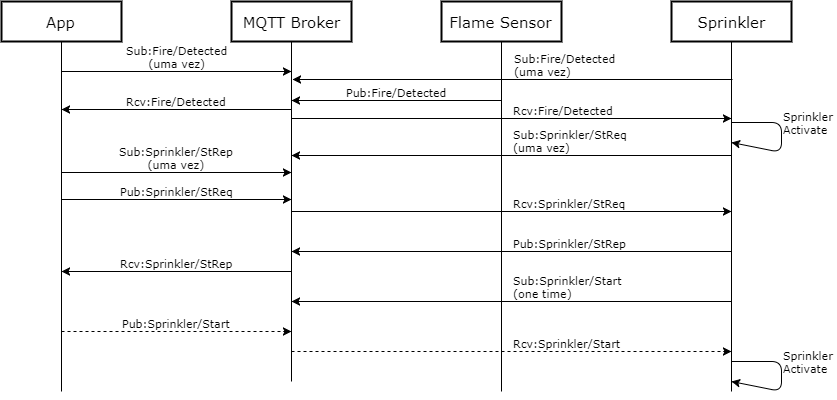
\includegraphics[width=1\textwidth]{imagens/projeto_msg.png}
	\caption{Procedimento de troca de mensagens do sistema IoT~\cite{kang2017room}, adaptado pelo autor.
		\label{fig:estudo_msg}}
\end{figure}
\FloatBarrier

Alguns elementos foram acrescentados na Figura~\ref{fig:estudo_msg} e na Tabela~\ref{tab:iot_protocol}, com a finalidade de deixá-las de acordo com as especificações do projeto. Ao descrever o cenário do aplicação,~\citeauthor{kang2017room} relatam que: "\textit{When the flame sensor detects the fire, the IoT device automatically alarms the fire event, activates the sprinkler to suppress the fire, and sends fire alarm message to smartphone app via IoT platform}". 

Observa-se que, os autores não deixam claro que o disparo do evento para ativação \textit{sprinkler} acontece mediante o recebimento de uma mensagem, que no caso, deve ser enviada pelo sensor de incêndio sob o tópico \textit{"Fire/Detected"}. 

Tanto na descrição do cenário quanto nos esquemas apresentados na Figura~\ref{fig:estudo_msg} e na Tabela~\ref{tab:iot_protocol}, o envio da mensagem de alerta de incêndio do sensor para o \textit{sprinkler} não é especificado. Sendo assim, foram adicionados procedimento para assinatura do tópico "\textit{Fire/Detected}" e recebimento do alerta por meio do tópico na Figura~\ref{fig:estudo_msg}, e a descrição do envio da mensagem na Tabela~\ref{tab:iot_protocol}.

Com base na descrição e objetivos do sistema, três processos que caracterizam seus compromissos são identificados: Detecção/Alerta; Checagem; e Supressão. Adiante, cada processo é modelado por meio da TPi de acordo com o comportamento operacional do MQTT quando QoS$=0$ e convertido em contrato multilateral por meio do algoritmo descrito na Seção~\ref{sec:algoritmo}. Por fim, o grafo de compromissos do sistema completo é obtido.

\section{Processo 1: Detecção/Alerta}

O processo de detecção e alerta de incêndio requer o envolvimento do sensor de incêndio, do \textit{Broker}, do aplicativo e do \textit{sprinkler}. Seu modelo em TPi é descrito como segue:
\begin{align}
& Sensor(FireDetection)~|~Broker()~|~App()~|~Sprinkler(),~em~que: \nonumber \\
& Sensor(z) \stackrel{def}{=} \overline{fd}\langle z \rangle \nonumber \\
& Broker() \stackrel{def}{=} fd(x).\overline{fd'}\langle x \rangle \nonumber \\
& App() \stackrel{def}{=} fd'(y) \nonumber \\
& Sprinkler() \stackrel{def}{=} fd'(y')
\end{align}

\subsection*{Aplicação do algoritmo}

O resultado obtido após a aplicação de cada passo do algoritmo é descrito como segue:
\begin{enumerate}
	\item $name$ = $C\_detectarIncêndio$;
	\item $Pi = (Sensor, FireDetection)$;
	\item $\mathcal{P} = \{Sensor, Broker, App, Sprinkler\}$;
	\item $\mathcal{D} = \{(Sensor, \{\overline{fd}\langle z \rangle\}), (Broker, \{fd(x).\overline{fd'}\langle x \rangle\}), (App, \{fd'(y)\}), (Sprinkler, \{fd'(y')\})\}$
	\item $\mathcal{A} = \{(\overline{fd}\langle z \rangle, Sensor), (fd(x), Broker), (\overline{fd'}\langle x \rangle, Broker), (fd'(y), App), (fd'(y'), Sprinkler)\}$
\end{enumerate}

De acordo com as regras estabelecidas na Seção~\ref{sec:algoritmo}, o compromisso pode ser declarado como:
\begin{eqnarray}
c_{1} = (C\_detectarIncendio, Sensor, Sprinkler, 5, \{&(\overline{fd}\langle z \rangle, tr), (fd(x), fi), (\overline{fd'}\langle x \rangle, tr), & \nonumber \\ &(fd'(y), fi), (fd'(y'), fi) \}) &
\end{eqnarray}

\section{Processo 2: Checagem}

O processo de checagem do status do \textit{sprinkler} requer o envolvimento do aplicativo, do \textit{broker} e do \textit{sprinkler}. Seu modelo em TPi é descrito a seguir:
\begin{align}
& App(SprinklerRequest)~|~Broker()~|~Sprinkler(),~em~que: \nonumber \\
& App(z) \stackrel{def}{=} \overline{req}\langle z \rangle . rep'(y) \nonumber \\
& Broker() \stackrel{def}{=} req(x) . \overline{req'}\langle x \rangle . rep(x') . \overline{rep'}\langle x' \rangle \nonumber \\
& Sprinkler() \stackrel{def}{=} req'(v) . \overline{rep}\langle reqReply \rangle
\end{align}

\subsection*{Aplicação do algoritmo}

O resultado obtido após a aplicação do algoritmo é exposto a seguir:
%alterar o Pi de dentro do () na descrição do algoritmo
\begin{enumerate}
	\item $name = C\_detectarIncendio$;
	\item $Pi = (App, SprinklerRequest)$;
	\item $\mathcal{P} = \{App, Broker, Sprinkler\}$
	\item $\mathcal{D} = \{ (App, \{\overline{req}\langle z \rangle . rep'(y)\}), (Broker, \{req(x) . \overline{req'}\langle x \rangle . rep(x') . \overline{rep'}\langle x' \rangle\}),$ 
	\\
	$(Sprinkler, \{req'(v) . \overline{rep}\langle reqReply \rangle\}) \};$
	\item $\mathcal{A} = \{ (\overline{req}\langle z \rangle, App), (req(x), Broker), (\overline{req'}\langle x \rangle, Broker), (req'(v), Sprinkler),
	\\
	(\overline{rep}\langle reqReply \rangle, Sprinkler), (rep(x'), Broker), (\overline{rep'}\langle x' \rangle, Broker), (rep'(y), App) \}.$
\end{enumerate}

Deste modo, o compromisso é definido como:
\begin{eqnarray}
c_{2} = (C\_checarStatus, App, App, 8,\{& (\overline{req}\langle z \rangle, tr), (req(x), fi), (\overline{req'}\langle x \rangle, tr)& \nonumber \\ 
&(req'(v), fi), (\overline{rep}\langle reqReply \rangle, tr), (rep(x'), fi), & \nonumber \\ 
&(\overline{rep'}\langle x' \rangle, tr), (rep'(y), fi) \} )&
\end{eqnarray}

\section{Processo 3: Supressão}

O processo de supressão de incêndio requer o envolvimento do sensor de incêndio, do Broker, do App e do Sprinkler. Seu modelo em TPi pode ser descrito abaixo:

\begin{align}
&Sensor(FireDetection)~|~Broker()~|~App()~|Sprinkler(),~em~que: \nonumber \\
&Sensor(z) \stackrel{def}{=} \overline{fd}\langle z \rangle \nonumber \\
&Broker \stackrel{def}{=} fd(x) . \overline{fd'}\langle x \rangle .  st(x') . \overline{st'}\langle x' \rangle \nonumber \\
&App() \stackrel{def}{=} fd'(s) . \overline{st}\langle startSprinkler \rangle  \nonumber \\
&Sprinkler() \stackrel{def}{=} st'(y)
\end{align}

\subsection*{Aplicação do algoritmo}

O resultado atingido após a aplicação do algoritmo é descrito a seguir:
\begin{enumerate}
	\item $name = C\_suprirIncendio$;
	\item $Pi = (Sensor, FireDetection)$;
	\item $\mathcal{P} = \{Sensor, Broker, App, Sprinkler\}$;
	\item $\mathcal{D} = \{ (Sensor, \{ \overline{fd}\langle z \rangle \nonumber \}), 
	(Broker, \{  fd(x) . \overline{fd'}\langle x \rangle .  st(x') . \overline{st'}\langle x' \rangle  \}), 
	\\
	(App, \{ fd'(s) . \overline{st}\langle startSprinkler \rangle \}), 
	(Sprinkler, \{ st'(y) \}) \};$
	\item $\mathcal{A} = \{ (\overline{fd}\langle z \rangle, Sensor), (fd(x), Broker), (\overline{fd'}\langle x \rangle, Broker), (fd'(s), App), 
	\\
	(\overline{st}\langle startSprinkler \rangle, App), (st(x'), Broker), (\overline{st'}\langle x' \rangle, Broker), (st'(y), Sprinkler) \}.$
\end{enumerate}

Assim, o compromisso é definido como segue:
\begin{eqnarray}
c_{3} = \{ C\_suprirIncendio, Sensor, Sprinkler, 8, \{& (\overline{fd}\langle z \rangle, tr), (fd(x), fi), & \nonumber \\  &(\overline{fd'}\langle x \rangle, tr) 
(fd'(s), fi), & \nonumber \\ & (\overline{st}\langle startSprinkler \rangle, tr), (st(x'), fi), & \nonumber \\ & (\overline{st'}\langle x' \rangle, tr), (st'(y), fi) \}&
\end{eqnarray}
\chapter{Trabalhos futuros}

-estudo mais profundo da modelagem em TPi para determinar a ordem de
execu��o dos sistemas, que ser�o a ordem de execu��o dos compromissos.

-definir mecanismo para definir a prioridade de execu��o quando uma a��o de sa�da tem mais de uma a��o de entrada
seguidas de uma ou mais a��es.

%%%% não esquece de deixar a impressão para imprimir só na frente%%%%%%%%%%%%%

% https://www.sinonimos.com.br/
% http://www.conjuga-me.net/
% https://www.significados.com.br/
% https://sci-hub.cc/
% http://citeseerx.ist.psu.edu/
% http://www.cesar.edu.br/qualis/
% http://libgen.io/
% ELEMENTOS PÓS-TEXTUAIS
% ----------------------------------------------------------
\postextual

\bibliography{bibliografia}

\end{document}
